\section{Difference in differences and panel event studies}\label{sec:A-did}

The last two sections of the appendix turn from estimators to research designs. Many questions in industrial
organization concern a discrete change in a market. Two firms merge, a rival
enters, a state raises a tax, or a patent is granted. A \emph{retrospective} (or ex post) evaluation measures
what the change did by comparing outcomes after it with outcomes before it. A \emph{prospective} (or ex ante)
evaluation predicts the effect before the change, with a model of demand, costs and conduct. This section
develops the research designs behind retrospectives. They compare units exposed to the change with units that
were not, before and after the change.

These designs are reduced form. They identify average effects of a change under assumptions about the outcomes
that units would have had without it, and they need no model of conduct. The book uses them for merger
retrospectives (\cref{sec:11-retro}), tax pass-through (\cref{sec:03-sumner}), entry
(\cref{sec:09-wc-did}) and patents (\cref{sec:05-dgg}). We build on the potential-outcomes notation of
\cref{sec:A-potential}. Throughout this section $i$ indexes units (products, markets, states, hospitals) and
$t$ indexes periods, and $\tau_t$ denotes a period fixed effect. In \cref{sec:A-eventstudy} the symbol $\tau$ will
index trading days instead.

\subsection{The two-by-two design}\label{sec:A-did-2x2}

We start with two groups and two periods. Units $i=1,\dots,n$ are observed in periods $t\in\{0,1\}$. The
indicator $\mathit{Treat}_i$ equals one for units in the \emph{treated group}, which is exposed to the change
between the two periods. The other units form the \emph{control group}. Let $\mathit{Post}_t=\indic\{t=1\}$ and
let $d_{it}=\mathit{Treat}_i\,\mathit{Post}_t$ be the treatment indicator. Each unit has two potential outcomes in
each period, $y_{it}(1)$ with the treatment and $y_{it}(0)$ without it. We observe
\begin{equation*}
y_{it}=y_{it}(0)+d_{it}\big[y_{it}(1)-y_{it}(0)\big].
\end{equation*}

\begin{definition}[Average effect of the treatment on the treated]\label{def:A-att}
The \emph{average treatment effect on the treated} in the post period, the panel version of the ATT of
\cref{sec:A-potential}, is
\begin{equation*}
\mathrm{ATT}=\E\big[y_{i1}(1)-y_{i1}(0)\mid \mathit{Treat}_i=1\big].
\end{equation*}
\end{definition}

Two naive comparisons fail. The cross-sectional comparison of treated and control units in period 1 adds a
selection term, the difference in untreated outcomes between the groups (\cref{prop:A-selection}). The
before-after comparison within the treated group adds the change that the treated units would have experienced
anyway:
\begin{equation*}
\E\big[y_{i1}-y_{i0}\mid\mathit{Treat}_i=1\big]=\mathrm{ATT}+\E\big[y_{i1}(0)-y_{i0}(0)\mid\mathit{Treat}_i=1\big],
\end{equation*}
provided that period-0 outcomes are untreated. A rise in input costs at the time of a merger, for example, is
attributed to the merger. The \emph{difference-in-differences} (DiD) estimator removes this change with the change
in the control group. Let $\bar y_{T,t}$ and $\bar y_{C,t}$ denote the sample means of $y_{it}$ in the treated and
control groups in period $t$. Then
\begin{equation}\label{eq:A-did-estimator}
\hat\beta^{\mathrm{DD}}=\big(\bar y_{T,1}-\bar y_{T,0}\big)-\big(\bar y_{C,1}-\bar y_{C,0}\big).
\end{equation}

\begin{assumption}[Identifying assumptions for DiD]\label{ass:A-did}
\leavevmode
\begin{enumerate}[label=(\roman*)]
\item \emph{No anticipation.} Period-0 outcomes are untreated: $y_{i0}=y_{i0}(0)$ for all $i$.
\item \emph{Parallel trends.} Without the treatment, the mean outcome would have changed by the same amount in both
groups:
\begin{equation*}
\E\big[y_{i1}(0)-y_{i0}(0)\mid\mathit{Treat}_i=1\big]=\E\big[y_{i1}(0)-y_{i0}(0)\mid\mathit{Treat}_i=0\big].
\end{equation*}
\item \emph{No interference.} The treatment of the treated group does not change the outcomes of control units:
$y_{i1}=y_{i1}(0)$ when $\mathit{Treat}_i=0$.
\end{enumerate}
\end{assumption}

\begin{proposition}[Identification by DiD]\label{prop:A-did}
Suppose the group means in \eqref{eq:A-did-estimator} are unbiased for the corresponding population means. Under
\cref{ass:A-did}, $\E[\hat\beta^{\mathrm{DD}}]=\mathrm{ATT}$. If the sample means are also consistent, then
$\hat\beta^{\mathrm{DD}}\xrightarrow{p}\mathrm{ATT}$.
\end{proposition}

\begin{proof}
Write $\E_1[\cdot]$ and $\E_0[\cdot]$ for expectations conditional on $\mathit{Treat}_i=1$ and
$\mathit{Treat}_i=0$. For the treated group, the observed outcome in period 1 is $y_{i1}(1)$, and by (i) the
period-0 outcome is $y_{i0}(0)$. Adding and subtracting $\E_1[y_{i1}(0)]$ gives
\begin{align*}
\E\big[\bar y_{T,1}-\bar y_{T,0}\big]
&=\E_1\big[y_{i1}(1)\big]-\E_1\big[y_{i0}(0)\big]\\
&=\E_1\big[y_{i1}(1)-y_{i1}(0)\big]+\E_1\big[y_{i1}(0)-y_{i0}(0)\big]\\
&=\mathrm{ATT}+\E_1\big[y_{i1}(0)-y_{i0}(0)\big].
\end{align*}
For the control group, (iii) and (i) give $\E[\bar y_{C,1}-\bar y_{C,0}]=\E_0[y_{i1}(0)-y_{i0}(0)]$. By (ii)
this equals the last term of the first display. Subtracting leaves $\mathrm{ATT}$. Consistency follows from the
continuous mapping theorem.
\end{proof}

The proof works for a panel, in which the same units appear in both periods, and for repeated cross sections. Two
features of the assumptions deserve comment. First, parallel trends restricts changes in outcomes and leaves their levels free. Suppose
untreated outcomes follow
\begin{equation}\label{eq:A-did-fe-model}
y_{it}(0)=\mu_i+\tau_t+\varepsilon_{it},\qquad \E\big[\varepsilon_{i1}-\varepsilon_{i0}\mid\mathit{Treat}_i\big]=0.
\end{equation}
Then $\E[y_{i1}(0)-y_{i0}(0)\mid\mathit{Treat}_i]=\tau_1-\tau_0$ in both groups, so (ii) holds however strongly the
unit effects $\mu_i$ are correlated with treatment. Firms that merge may have higher prices to begin with. What DiD
needs is that their prices would not have grown faster.

Second, parallel trends depends on the scale of the outcome. Suppose the control mean of the untreated outcome
rises from 10 to 11 and the treated mean would have risen from 20 to 21. Trends are parallel in levels. In logs the
control change is $\ln\frac{11}{10}\approx0.095$ and the treated change is $\ln\frac{21}{20}\approx0.049$, so trends
are not parallel. Merger retrospectives usually work with log prices. Their assumption is that, absent the merger,
the proportional price changes of the two groups would have been equal.

\casehead{Regression form}
The same estimate comes from the regression
\begin{equation}\label{eq:A-did-reg}
y_{it}=\alpha+\gamma\,\mathit{Treat}_i+\lambda\,\mathit{Post}_t+\beta^{\mathrm{DD}}\,\mathit{Treat}_i\mathit{Post}_t+e_{it}.
\end{equation}
The four regressors span the four group-period cells, so OLS fits each cell mean exactly:
\begin{align*}
\hat\alpha&=\bar y_{C,0}, & \hat\alpha+\hat\lambda&=\bar y_{C,1},\\
\hat\alpha+\hat\gamma&=\bar y_{T,0}, & \hat\alpha+\hat\gamma+\hat\lambda+\hat\beta^{\mathrm{DD}}&=\bar y_{T,1}.
\end{align*}
Subtract the second equation from the fourth and the first from the third. The difference of the two results is
$\hat\beta^{\mathrm{DD}}=(\bar y_{T,1}-\bar y_{T,0})-(\bar y_{C,1}-\bar y_{C,0})$. In a balanced panel we can
replace $\alpha+\gamma\,\mathit{Treat}_i$ by unit fixed effects $\mu_i$. Differencing the two periods then gives
\begin{equation*}
y_{i1}-y_{i0}=\lambda+\beta^{\mathrm{DD}}\,\mathit{Treat}_i+(e_{i1}-e_{i0}).
\end{equation*}
The OLS slope on a binary regressor is the difference in group means of the dependent variable, which is again
\eqref{eq:A-did-estimator}. The regression form is convenient for standard errors (\cref{sec:A-did-inference}) and for
adding covariates. With covariates, the assumption becomes \emph{conditional parallel trends}: (ii) holds within
cells of baseline covariates $x_i$. The regression then interacts $x_i$ with $\mathit{Post}_t$. Covariates that the
treatment itself changes should not be included, because they absorb part of the effect.

\Cref{fig:A-did} shows the design with several periods on each side of the change. The pre-period paths are
parallel. After adoption the treated path jumps. The dashed line continues the treated path at the slope of the
control path, which is the counterfactual implied by parallel trends. The vertical gap between the observed and
counterfactual paths is the ATT.

\begin{figure}[htbp]
\centering
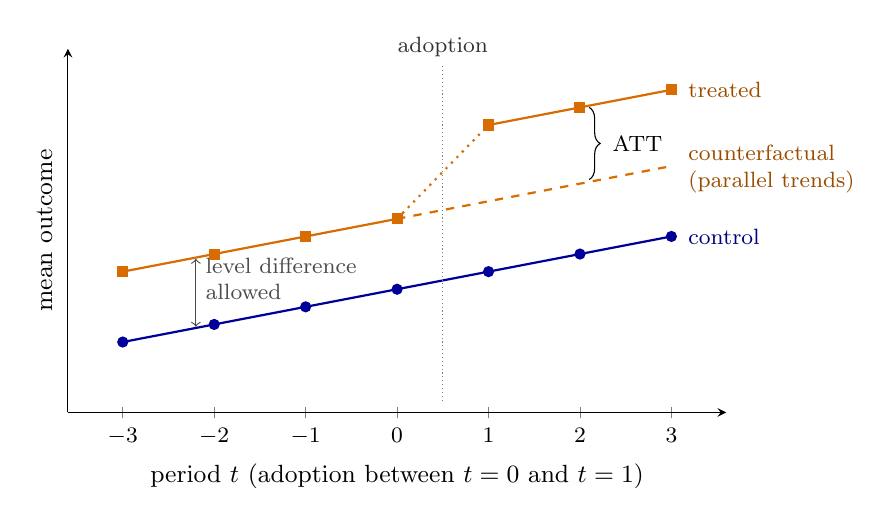
\begin{tikzpicture}
\begin{axis}[
  width=0.82\textwidth, height=6.2cm,
  xmin=-3.6, xmax=3.6, ymin=0, ymax=6.2,
  axis lines=left, xtick={-3,-2,-1,0,1,2,3}, ytick=\empty,
  xlabel={period $t$ (adoption between $t=0$ and $t=1$)}, ylabel={mean outcome},
  xlabel style={font=\small}, ylabel style={font=\small}, tick label style={font=\footnotesize},
  clip=false]
\addplot[thick, blue!60!black, mark=*, mark size=1.6pt, domain=-3:3, samples=7] {1.2+0.3*(x+3)};
\addplot[thick, orange!85!black, mark=square*, mark size=1.6pt, domain=-3:0, samples=4] {2.4+0.3*(x+3)};
\addplot[thick, orange!85!black, mark=square*, mark size=1.6pt, domain=1:3, samples=3] {2.4+0.3*(x+3)+1.3};
\addplot[thick, orange!85!black, dotted, domain=0:1, samples=2] {2.4+0.3*(x+3)+1.3*x};
\addplot[thick, dashed, orange!85!black, domain=0:3, samples=4] {2.4+0.3*(x+3)};
\draw[gray, densely dotted] (axis cs:0.5,0.2) -- (axis cs:0.5,5.9);
\node[font=\footnotesize, gray!40!black, anchor=south] at (axis cs:0.5,5.9) {adoption};
\draw[decorate, decoration={brace, mirror, amplitude=4pt}] (axis cs:2.1,3.97) -- (axis cs:2.1,5.2)
  node[midway, right=5pt, font=\footnotesize] {$\mathrm{ATT}$};
\node[font=\footnotesize, orange!60!black, anchor=west] at (axis cs:3.08,5.5) {treated};
\node[font=\footnotesize, orange!60!black, anchor=west, align=left] at (axis cs:3.08,4.15)
  {counterfactual\\(parallel trends)};
\node[font=\footnotesize, blue!50!black, anchor=west] at (axis cs:3.08,3.0) {control};
\draw[<->, gray!60!black] (axis cs:-2.2,1.46) -- (axis cs:-2.2,2.62)
  node[midway, right, yshift=5pt, font=\footnotesize, align=left] {level difference\\allowed};
\end{axis}
\end{tikzpicture}
\caption{The difference-in-differences design. Squares are the mean outcomes of the treated group and dots those
of the control group. The dashed line is the treated group's untreated path implied by parallel trends. The vertical
distance between the observed treated path and the dashed line is the average effect on the treated. Groups may
differ in levels.}
\label{fig:A-did}
\end{figure}

\subsection{Two-way fixed effects and continuous treatment}\label{sec:A-did-twfe}

With many periods, and possibly a treatment of varying intensity, the DiD regression generalizes to the
\emph{two-way fixed-effects} (TWFE) model
\begin{equation}\label{eq:A-twfe}
y_{it}=\mu_i+\tau_t+\beta\,d_{it}+e_{it},\qquad i=1,\dots,n,\quad t=1,\dots,T,
\end{equation}
where $d_{it}$ may be binary or continuous. The unit effects $\mu_i$ absorb permanent differences across units, and
the period effects $\tau_t$ absorb shocks common to all units in a period.

Let $\tilde d_{it}$ be the residual from regressing $d_{it}$ on the unit and period dummies. By the
Frisch-Waugh-Lovell theorem (\cref{thm:A-fwl}), the OLS estimate of $\beta$ equals the slope of a regression of
$y_{it}$ on $\tilde d_{it}$:
\begin{equation}\label{eq:A-twfe-fwl}
\hat\beta=\frac{\sum_{i,t}\tilde d_{it}\,y_{it}}{\sum_{i,t}\tilde d_{it}^2}.
\end{equation}
In a balanced panel the residual has the closed form already used in \cref{sec:A-panel}. Let $\bar d_i$, $\bar d_t$ and $\bar d$ be the unit, period and
overall means of $d_{it}$. Then
\begin{equation}\label{eq:A-dtilde}
\tilde d_{it}=d_{it}-\bar d_i-\bar d_t+\bar d.
\end{equation}
To verify \eqref{eq:A-dtilde}, note two facts. The difference $d_{it}-\tilde d_{it}=\bar d_i+\bar d_t-\bar d$ is a
unit term plus a period term, so it lies in the span of the dummies. And $\tilde d_{it}$ sums to zero over $t$ for
each $i$ and over $i$ for each $t$, so it is orthogonal to every dummy. These are the two properties that define the
residual of a projection.

\casehead{Identification}
Substitute \eqref{eq:A-twfe} into \eqref{eq:A-twfe-fwl}. The fixed effects drop out because
$\sum_{i,t}\tilde d_{it}(\mu_i+\tau_t)=0$, and $\sum_{i,t}\tilde d_{it}d_{it}=\sum_{i,t}\tilde d_{it}^2$ because
$\tilde d_{it}$ is orthogonal to $d_{it}-\tilde d_{it}$. Hence
\begin{equation*}
\hat\beta=\beta+\frac{\sum_{i,t}\tilde d_{it}\,e_{it}}{\sum_{i,t}\tilde d_{it}^2}.
\end{equation*}
Let $\mathbf{d}$ collect the treatments of all units in all periods. If $\E[e_{it}\mid\mathbf{d}]=0$ for every $i$
and $t$, then $\E[\hat\beta\mid\mathbf{d}]=\beta$. This \emph{strict exogeneity} condition is the multi-period form of
parallel trends and no anticipation. It allows treatment to be correlated with $\mu_i$. It rules out treatment
that responds to past or expected future shocks to the unit's outcome.

The variation that identifies $\beta$ is the change in a unit's treatment relative to the average change across
units. The two-unit, two-period case shows this transparently. Let units $A$ and $B$ be observed in two periods, and
write $\Delta y_i=y_{i2}-y_{i1}$ and $\Delta d_i=d_{i2}-d_{i1}$. First differences remove $\mu_i$:
\begin{equation*}
\Delta y_i=(\tau_2-\tau_1)+\beta\,\Delta d_i+\Delta e_i,\qquad i\in\{A,B\}.
\end{equation*}
Two equations in two unknowns fit exactly. Subtracting the equation for $B$ from that for $A$ gives
\begin{equation}\label{eq:A-wald-did}
\hat\beta=\frac{\Delta y_A-\Delta y_B}{\Delta d_A-\Delta d_B}.
\end{equation}
The estimate is the DiD in outcomes divided by the DiD in treatment. It has the form of a Wald estimator
(\cref{sec:A-iv}), with the change in treatment playing the role of the first stage.

\casehead{Sumner's tax regression as a DiD with a continuous dose}
The cigarette regression of \citet{Sumner1981}, written as \eqref{eq:A-sumner} in \cref{sec:A-panel}, is a TWFE
regression with a continuous treatment, the specific tax $t_{sy}$ of state $s$ in year $y$. The pass-through $\rho$
equals one under competition with constant marginal cost and exceeds one under market power with constant-elasticity
demand (\cref{sec:03-passthrough-theory}). By \eqref{eq:A-wald-did}, a state that raises its tax by 10 cents more than
another state identifies $\rho$ from the difference in their price changes. Sumner states the identifying assumption
directly. The remaining price variation ``is assumed to be uncorrelated with $R_{it}$'' (p.~1015), where $R_{it}$ is his
notation for the tax. He adds that the state dummies account for any stable pattern of state tax rates, such as an
effect of the unchanging location of the tobacco industry (pp.~1015--1016).

\Cref{sec:A-panel} reports his estimates. The two-way estimate of 1.074 falls to 1.029 when the year effects are
replaced by the national price index and the state effects are dropped. Cross-state differences in tax levels and
within-state tax changes therefore carry different information. The main threats to \eqref{eq:A-sumner} are tax
increases timed with changes in local demand or cost, and cross-border purchases that make legal sales respond to the
tax gap with neighboring states. Sumner checks the second by adding a squared tax term to year-by-year regressions. It
is insignificant in most years (n.~9, p.~1017). \Cref{sec:A-sumner-se} shows that the standard error of $\hat\rho$ more
than doubles once dependence within states is allowed.

\begin{remark}[Heterogeneous pass-through]\label{rem:A-twfe-hetero}
Suppose pass-through differs across states, so that $p_{sy}=\mu_s+\tau_y+\rho_s t_{sy}+e_{sy}$ with strictly
exogenous errors. Repeating the steps above gives $\E[\hat\rho\mid\mathbf{t}]=\sum_sW_s\rho_s$ with
\begin{equation*}
W_s=\frac{\sum_y\tilde t_{sy}\,t_{sy}}{\sum_{s',y}\tilde t_{s'y}^2},\qquad \sum_sW_s=1 .
\end{equation*}
In a balanced panel $\sum_y\tilde t_{sy}=0$, so we may replace $t_{sy}$ by $t_{sy}-\bar t_s$, and
$t_{sy}-\bar t_s=\tilde t_{sy}+(\bar t_y-\bar t)$ by \eqref{eq:A-dtilde}. Therefore
\begin{equation*}
W_s=\frac{\sum_y\tilde t_{sy}^2+\sum_y\tilde t_{sy}\,(\bar t_y-\bar t)}{\sum_{s',y}\tilde t_{s'y}^2}.
\end{equation*}
The first term is the state's share of the residual tax variation. The second term sums to zero across states, but
it can be negative for a state whose tax deviations move against the national path. A weight can then be negative.
\citet{CallawayGoodmanBaconSantAnna2024} show that with a continuous dose the TWFE coefficient also mixes effects at
different dose levels. Comparing units with different doses then needs a stronger assumption than parallel trends.
\end{remark}

\subsection{Control groups in IO retrospectives}\label{sec:A-did-control}

A good control group satisfies two requirements. It is subject to the same shocks as the treated group, so that
parallel trends is plausible. And it is unaffected by the treatment, so that no interference holds. In product
markets these requirements pull in opposite directions. Products that share the demand and cost shocks of the
merging products are their close substitutes, and close substitutes respond to the merger. With Bertrand
competition prices are strategic complements, so rivals raise their prices when the merged firm raises its own.
The next proposition shows what this does to the estimate.

\begin{proposition}[Partially affected controls]\label{prop:A-did-spillover}
Let (i) and (ii) of \cref{ass:A-did} hold, and suppose that the treatment raises the mean outcome of the control
group by a fraction $\kappa$ of the effect on the treated:
\begin{equation*}
\E\big[y_{i1}-y_{i1}(0)\mid\mathit{Treat}_i=0\big]=\kappa\cdot\mathrm{ATT}.
\end{equation*}
Then $\E[\hat\beta^{\mathrm{DD}}]=(1-\kappa)\mathrm{ATT}$. If $0\le\kappa<1$, the expectation of the DiD estimate has
the sign of the ATT and is no larger in magnitude. It is then a lower bound on the size of the effect. If $\kappa=1$,
the expectation is zero. If $\kappa<0$, DiD overstates the effect.
\end{proposition}

\begin{proof}
The treated-group change is as in the proof of \cref{prop:A-did}:
$\E[\bar y_{T,1}-\bar y_{T,0}]=\mathrm{ATT}+\E_1[y_{i1}(0)-y_{i0}(0)]$. For the control group, add and subtract
$\E_0[y_{i1}(0)]$ and use (i):
\begin{align*}
\E\big[\bar y_{C,1}-\bar y_{C,0}\big]
&=\E_0\big[y_{i1}-y_{i1}(0)\big]+\E_0\big[y_{i1}(0)-y_{i0}(0)\big]\\
&=\kappa\cdot\mathrm{ATT}+\E_0\big[y_{i1}(0)-y_{i0}(0)\big].
\end{align*}
Subtract the second display from the first and use (ii) to cancel the trends. The result is
$(1-\kappa)\mathrm{ATT}$. For $0\le\kappa\le1$ the factor $1-\kappa$ lies in $[0,1]$, which gives the bound. For
$\kappa<0$ the factor exceeds one.
\end{proof}

The fraction $\kappa$ has a structural interpretation. Consider a symmetric linear Bertrand oligopoly with $N$ firms,
two of which merge, with own-price demand slope $b$ and cross-price slope $d$. \Cref{prop:11-didbias} shows that each
outsider raises its price by $\kappa=\frac{2d}{2b-(N-3)d}$ times the insiders' increase. With three firms $\kappa$ equals the diversion ratio between the merging products. The bias is
therefore largest when the merging products are close substitutes, which is when the merger matters most. A
negative $\kappa$ arises for quantities. If the merged firm raises its prices, rivals gain sales, and a DiD in
quantities with rivals as controls overstates the merging firms' loss.

The opposite choice, a distant control, has the opposite problem. Store brands (private labels) use the same
inputs as branded products, and if they are supplied elastically their prices track costs while the merger leaves
them alone, so $\kappa\approx0$. But they may face different demand shocks. A rise in income can raise the demand for
branded goods relative to store brands. Then (ii) fails and the private-label estimate is biased in an unknown
direction. Reporting both control groups shows how much the conclusion depends on this trade-off. We now look at
five designs from the book. \Cref{tab:A-did-apps} summarizes them, with Sumner's design for comparison.

\casehead{Ashenfelter and Hosken (2010): two control groups}
\citet{AshenfelterHosken2010} study five consumer-product mergers that looked problematic from the public record
(\cref{sec:11-ah}).\footnote{We use the NBER working-paper version, \citet{AshenfelterHosken2008}, for page and table
numbers.} For each merging product and its control group they estimate, in logs,
\begin{equation}\label{eq:A-ah}
p_{ijt}=\alpha_{ij}+\sum_{m=1}^{11}\delta_m M_{ijt}+\beta_1\,\mathit{Post}_{ijt}
+\beta_2\,\mathit{Post}_{ijt}\times\mathit{MergingParty}_i+e_{ijt},
\end{equation}
for product $i$ in city $j$ and month $t$ (their eq.~1, p.~24). Here $\alpha_{ij}$ is a product-city fixed effect and
$M_{ijt}$ are calendar-month indicators for seasonality. The coefficient $\beta_2$ is the DiD estimate of the
proportional price change. The preferred control group is the private-label products closest to the merging brands.
The alternative is branded close substitutes, which the authors expect to understate the effect for the reason in
\cref{prop:A-did-spillover} and treat mainly as a specification check (pp.~23--24). The preferred window has equal
spans of data before and after the merger and drops the three months on each side of consummation (p.~22). Dropping
those months avoids having to date the start of joint pricing. The symmetric window guards against transitory
selection, a point first made by \citet{HeckmanRobb1985} and used by \citet{AshenfelterCard1985}
(\cref{prop:11-window}).

The aggregate effects in their Table~13 show that the control group matters (\cref{tab:11-ah}). With private-label
controls, Pennzoil and Quaker State raised prices by 0.052 log points (s.e.\ 0.013), against 0.014 (0.011) with
branded controls. For Procter and Gamble and Tambrands the figures are 0.070 (0.008) and 0.023 (0.007). Both
patterns fit \cref{prop:A-did-spillover} with $\kappa$ between zero and one. For General Mills and the Chex brands
the order reverses, 0.032 (0.005) against 0.057 (0.005). If private-label prices were unaffected and followed
parallel trends, \cref{prop:A-did-spillover} would make the branded estimate the smaller one. The reversal therefore
means that at least one control group violates the assumptions, through different trends or through store-brand
prices that responded to the merger.

\casehead{Ashenfelter, Hosken and Weinberg (2013): composition and product turnover}
\citet{AshenfelterHoskenWeinberg2013} study the 2006 Whirlpool-Maytag merger in major appliances
(\cref{sec:11-maytag}).\footnote{We use the NBER working-paper version, \citet{AshenfelterHoskenWeinberg2011}, for page
numbers.} The treated categories are dishwashers, refrigerators, clothes washers and clothes dryers. The comparison
categories are cooktops, freezers, ovens and ranges, restricted to brands not made by either party, where the merger
changed concentration little (p.~10). Their eq.~(4) (p.~12) is
\begin{equation}\label{eq:A-ahw4}
\begin{split}
\ln p_{it}={}&\beta_1\,\mathit{Maytag}_i\times\mathit{Post}_t+\beta_2\,\mathit{Whirlpool}_i\times\mathit{Post}_t\\
&+\sum_k\gamma^T_k\mathit{Age}^T_{ikt}+\sum_k\gamma^C_k\mathit{Age}^C_{ikt}+\sum_l\lambda_l\,\mathit{Month}_{lt}+\alpha_i+e_{it},
\end{split}
\end{equation}
where $i$ is a stock-keeping unit (SKU), a narrowly defined model, and $\alpha_i$ an SKU fixed effect. The age
indicators are separate for treatment and comparison categories, because appliance prices fall with a model's age at
category-specific rates. The month effects absorb common shocks.

Product turnover creates a composition problem with a sharp econometric form. For an SKU introduced after the merger,
$\mathit{Post}_t=1$ in every month it is observed. Its interaction $\mathit{Maytag}_i\times\mathit{Post}_t$ then
equals the constant $\mathit{Maytag}_i$ and is absorbed by $\alpha_i$. With SKU effects, the merger effect is
identified only from SKUs sold both before and after the merger (p.~13). Since most models live about a year, this
discards the products introduced after the merger, whose prices the merged firm chose. The authors' eq.~(5) replaces
$\alpha_i$ by observed characteristics and brand dummies, so new SKUs contribute. On SKUs introduced within a year of
the merger, eqs.~(4) and~(5) give nearly identical effects (pp.~14--15). The authors read this agreement as evidence
that unobserved SKU quality is not correlated with the post-merger indicators, given the characteristics. The preferred results
show price increases for new products in two categories. New Whirlpool dryers rose by 13 to 17 percent, depending on
the comparison category, and new Maytag dishwashers by 5 to 7 percent (p.~16). Standard errors are clustered by SKU
(p.~14).

\casehead{Bj\"ornerstedt and Verboven (2016): merging firms against rivals}
\citet{BjornerstedtVerboven2016} evaluate the acquisition of AstraZeneca Tika (AZT) by GlaxoSmithKline (GSK) in the
Swedish market for painkillers (\cref{sec:11-bv}).\footnote{Only pp.~134, 137 and 147 of the published article were
available to us. References marked WP are to the January 2013 working paper, \citet{BjornerstedtVerboven2013}. Its
printed page numbers equal its PDF page numbers minus one.} The two firms were the only sellers of paracetamol, and
the Swedish Competition Authority cleared the merger on April 3, 2009 (WP pp.~4 and~6). Their retrospective
regression, in the spirit of \eqref{eq:A-ah}, is
\begin{equation*}
\ln p_{gt}=\alpha_g+\beta_g\,\mathit{PostMerger}_t+e_{gt},
\end{equation*}
where $p_{gt}$ is the average price of product group $g$ in month $t$ (eq.~1, p.~134, and WP eq.~18). Each group
has its own post-merger change. \citet{AshenfelterHosken2010} instead give all control products a common change
(WP p.~27, n.~16). The difference between the merging group's $\beta_g$ and a rival group's $\beta_g$ is a DiD
estimate. The authors note that the merger may also raise rival prices, and the difference is then a lower bound for
the merger effect (p.~134). This is the case $0<\kappa<1$ of \cref{prop:A-did-spillover}.

The two versions of the paper use different windows. The published article defines groups by substance and by
substance and firm. It compares one year before with one year after the merger, ``to exclude possible changes after
the deregulation'' of the Swedish pharmacy monopoly (p.~134). The working paper compares April 2007 to April 2009
with May 2009 to May 2011, and reports groups by substance and by firm (WP pp.~27--28). In that longer window the
paracetamol price drifts down near the end, ``perhaps associated with new entry threats following the deregulation''
(WP p.~27). The one-year window of the published article leaves out these months.

The regression table of the published article (its Table~4, one-year window) was not available to us. We therefore
report WP Table~7, which uses the two-year window and robust standard errors. The published estimates may differ. In
log points, the post-merger change is 0.351 (0.007) for paracetamol, 0.001 (0.005) for ibuprofen and 0.100 (0.004)
for acetylsalicylic acid (ASA, sold as aspirin). The merging firms moved together, with 0.356 (0.006) for AZT and
0.379 (0.009) for GSK. With ibuprofen as the control group, the DiD estimate is 0.350 log points, or 42 percent.
With ASA as the control, it is 0.251, or 29 percent (WP p.~29). Pooling the two rival substances into one control
gives 0.30, or 35 percent (WP p.~29, n.~17). The abstract of the working paper reports these figures as an increase of 42
percent in absolute terms and 35 percent relative to rivals. The ASA increase fits $\kappa>0$, which makes the
ASA-based estimate the smaller one. The authors offer a second reason, a mandated cut in ASA package sizes (WP
p.~29). That reason is a failure of parallel trends instead. Both reasons lower the ASA-based estimate, and the
design cannot separate them.

\casehead{Dafny (2009): rival exposure, an instrument and placebo periods}
\citet{Dafny2009} measures the effect of hospital mergers on the prices of rival hospitals (\cref{sec:11-dafny}).
\Cref{sec:A-ivmodel} sets out her design. Read as a panel design, it is a first-differenced TWFE model with a
continuous treatment. The unit is a hospital that did not merge, and the outcome is the long difference in log price
from 1988 to 1997. The treatment is the number of rival mergers between 1989 and 1996, as in \eqref{eq:A-dafny-iv}.
Strict exogeneity fails here. Hospitals with merging rivals had slower price growth before the merger wave
(\cref{sec:A-potential}), so mergers happened in markets on different paths. The co-location instrument restores
identification, and \cref{tab:A-dafny} reports the first stage, the reduced form and the IV and OLS estimates.

The design borrows the event-study logic of \cref{sec:A-did-es} through placebo periods. If co-location affected
price growth through channels other than mergers, it would also predict growth before and after the merger wave.
The reduced-form coefficient is $-0.016$ (0.010) for 1985--1988 and $-0.008$ (0.013) for 1997--2000 (panel B of
\cref{tab:A-dafny}). These are tests of the exclusion restriction in the spirit of pre-trend tests.

\casehead{Whinston and Collins (1992): two cohorts as each other's controls}
\citet{WhinstonCollins1992} study incumbent responses to entry by People Express on routes out of Newark
(\cref{sec:09-wc-did}). Markets entered in 1984 and markets entered in 1985 are observed in the first quarters of
1984, 1985 and 1986. Let $D_{my}=1$ if market $m$ has been entered by year $y$, and consider
\begin{equation*}
\ln P_{my}=\mu_m+\nu_y+\beta\,D_{my}+e_{my}.
\end{equation*}
For the 1984 cohort $D$ is $(0,1,1)$ across the three years, and for the 1985 cohort it is $(0,0,1)$. In 1984--1985
the 1985 cohort, not yet entered, is the control for the 1984 cohort. In 1985--1986 the 1984 cohort, already entered,
is the control for the 1985 cohort. The incumbents' mean price fell 33 percent (s.d.\ 26) in the 1984 cohort and rose
2 percent (24) in the 1985 cohort during 1984--1985, with a two-sample $t$ statistic of 2.5. In 1985--1986 the
changes were 0 percent (15) and $-35$ percent (21), with $t=3.5$ (Table~3, p.~459). The second comparison uses an
already treated group as control. It is valid only if the 1984 cohort's effect stayed constant in its second year.
The flat 1984 cohort change in 1985--1986 supports that assumption. \Cref{sec:A-did-staggered} shows why this
condition matters in staggered designs. The authors also caution that demand or cost conditions may have changed in
the entered markets, and could even have caused entry (pp.~458--459).

\begin{remark}[DiD inside a structural model]\label{rem:A-did-structural}
\citet[pp.~1779--1780]{MillerWeinberg2017} estimate a supply model for beer that allows a departure from Nash-Bertrand
after the merger. ABI and MillerCoors may then partly or fully internalize the effect of their prices on each other's
profits. The instrument that identifies the departure is an indicator for ABI and MillerCoors products after the
merger. A separate post-merger cost shifter for MillerCoors isolates the comparison between ABI and the imported brands of Modelo and Heineken.
Identification therefore rests on a DiD comparison of implied marginal costs, which \cref{prop:11-mc-did} makes
exact. Parallel trends is then an assumption about the unobserved costs of ABI and of the imported brands.
\end{remark}

\begin{table}[htbp]
\centering
\caption{Difference-in-differences designs in the book}
\label{tab:A-did-apps}
\footnotesize
\begin{tabularx}{\textwidth}{@{}>{\raggedright\arraybackslash}p{2.05cm}>{\raggedright\arraybackslash}X>{\raggedright\arraybackslash}X>{\raggedright\arraybackslash}p{2.2cm}>{\raggedright\arraybackslash}p{1.9cm}>{\raggedright\arraybackslash}X@{}}
\toprule
Study & Treatment & Control & Window & Inference & Main threat\\
\midrule
\citet{Sumner1981} & state-year cigarette tax (continuous) & tax changes in other states, via state and year effects & annual, 1954--1978 & conventional, and random effects & taxes timed with local shocks, cross-border sales\\
\addlinespace
\citet{AshenfelterHosken2010} & five consumer-product mergers & private labels (preferred) or branded substitutes & symmetric, 3 months dropped on each side & clustered by month & rival responses, store-brand demand shocks\\
\addlinespace
\citet{AshenfelterHoskenWeinberg2013} & Whirlpool-Maytag, four appliance categories & cooktops, freezers, ovens, ranges of other brands & SKUs in their first year, monthly & clustered by SKU & product turnover and composition\\
\addlinespace
\citet{BjornerstedtVerboven2016} & paracetamol merger, Sweden, 2009 & ibuprofen and ASA groups & one year before and after (published), two years (WP) & robust s.e.\ (WP Table~7) & rival responses, ASA package sizes, deregulation\\
\addlinespace
\citet{Dafny2009} & number of rival hospital mergers, 1989--1996 & hospitals with fewer rival mergers, with a co-location instrument & long difference 1988--1997, placebos 1985--1988 and 1997--2000 & IV, Hausman test & co-location related to price growth\\
\addlinespace
\citet{WhinstonCollins1992} & People Express entry, Newark markets & markets entered in the other year & first quarters 1984, 1985, 1986 & two-sample $t$, 13 d.f. & entry timed with market shocks, changing effects\\
\bottomrule
\end{tabularx}

\smallskip
\parbox{\textwidth}{\footnotesize Notes: Entries are taken from the papers' text and tables, cited in the main
text. ASA is acetylsalicylic acid. For Bj\"ornerstedt and Verboven, the one-year window is that of the published
article (p.~134). The two-year window and the inference come from the January 2013 working paper (WP).}
\end{table}

\casehead{Which mergers are studied}
A retrospective estimates the effect of one merger. Conclusions about mergers in general also depend on which
mergers are studied, and \citet[pp.~255--256]{AskerNocke2021} list three filters. The studied mergers were
consummated, so an antitrust authority had usually cleared them, and blocked or deterred mergers are missing. They
come from industries with good data, mostly consumer-facing ones, and few concern intermediate goods. They also tend
to be large or to illustrate a phenomenon of interest. In potential-outcomes terms, an average over studied mergers is
an ATT for a selected population. It need not equal the effect of a merger that the authority would have blocked.
Their survey of retrospectives published from 2000 to 2020 finds a wide range of price effects. Some prices rose
sharply, some did not move and some fell (pp.~256--257).

\subsection{Inference}\label{sec:A-did-inference}

DiD data are panels, and panel errors are dependent. Outcomes of a unit are correlated over time, and outcomes of
units in the same period share common shocks. Which dependence matters depends on the regressors in the model. We
treat serial correlation first.

\begin{proposition}[DiD as a comparison of unit-level changes]\label{prop:A-did-collapse}
Consider a balanced panel with $T_0$ pre-periods and $T_1$ post-periods, a common adoption date, $n_1$ treated and
$n_0$ control units. Let $\Delta_i=\bar y_{i,\mathrm{post}}-\bar y_{i,\mathrm{pre}}$ be unit $i$'s change in mean
outcome. The TWFE estimate of $\beta$ in \eqref{eq:A-twfe} with $d_{it}=\mathit{Treat}_i\mathit{Post}_t$ equals
\begin{equation*}
\hat\beta=\bar\Delta_1-\bar\Delta_0,
\end{equation*}
the difference between the mean changes of treated and control units. If units are independent, then
$\Var(\hat\beta\mid\mathit{Treat})=\frac{\sigma_{\Delta,1}^2}{n_1}+\frac{\sigma_{\Delta,0}^2}{n_0}$, with
$\sigma_{\Delta,g}^2$ the variance of $\Delta_i$ in group $g$, whatever the serial correlation within units.
\end{proposition}

\begin{proof}
Let $p=\frac{n_1}{n}$ and $q=\frac{T_1}{T}$. With a common adoption date, $\bar d_i=q\,\mathit{Treat}_i$,
$\bar d_t=p\,\mathit{Post}_t$ and $\bar d=pq$. By \eqref{eq:A-dtilde},
\begin{equation*}
\tilde d_{it}=\mathit{Treat}_i\mathit{Post}_t-q\,\mathit{Treat}_i-p\,\mathit{Post}_t+pq=(\mathit{Treat}_i-p)(\mathit{Post}_t-q).
\end{equation*}
The denominator of \eqref{eq:A-twfe-fwl} is $\sum_i(\mathit{Treat}_i-p)^2\sum_t(\mathit{Post}_t-q)^2=np(1-p)\cdot Tq(1-q)$.
For the numerator, first sum over periods:
\begin{equation*}
\sum_t(\mathit{Post}_t-q)\,y_{it}=T_1(1-q)\,\bar y_{i,\mathrm{post}}-T_0\,q\,\bar y_{i,\mathrm{pre}}=Tq(1-q)\,\Delta_i,
\end{equation*}
using $T_1=qT$ and $T_0=(1-q)T$. Then sum over units:
$\sum_i(\mathit{Treat}_i-p)\Delta_i=np\bar\Delta_1-p(np\bar\Delta_1+n(1-p)\bar\Delta_0)=np(1-p)(\bar\Delta_1-\bar\Delta_0)$.
Dividing gives $\hat\beta=\bar\Delta_1-\bar\Delta_0$. The variance follows because the $\Delta_i$ are independent
across units.
\end{proof}

The proposition gives the right standard error in two equivalent ways. We may collapse the data to one change per
unit and compare means, or cluster the TWFE regression by unit (\cref{sec:A-cluster}). Conventional OLS standard errors
treat the $nT$ errors as independent, and they are too small when errors are positively autocorrelated. Suppose the
errors of each unit follow a stationary AR(1) process with coefficient $r$ and variance $\sigma^2$. The variance of a
mean of $m$ consecutive errors is
\begin{equation*}
\Var\Big(\frac{1}{m}\sum_{t=1}^{m}e_{it}\Big)=\frac{\sigma^2}{m^2}\Big[m+2\sum_{h=1}^{m-1}(m-h)\,r^h\Big]
\approx\frac{\sigma^2}{m}\cdot\frac{1+r}{1-r}
\end{equation*}
for large $m$, since $\sum_{h=-\infty}^{\infty}r^{|h|}=\frac{1+r}{1-r}$. The covariance between the pre-period and
post-period means is of order $\frac{1}{m^2}$ and becomes negligible. The independence formula therefore understates
the variance of $\Delta_i$ by a factor of about $\frac{1+r}{1-r}$, which is 9 when $r=0.8$. The standard error is
then too small by a factor of 3. This is the mechanism behind the placebo evidence of
\citet{BertrandDufloMullainathan2004} discussed in \cref{sec:A-cluster}. Clustering by state or collapsing to pre and
post means fixes the problem when there are many states.

\casehead{Few treated units}
Cluster-robust inference relies on many clusters, and in particular on many treated clusters. Retrospectives often
have one merger, or a handful of treated markets. \citet{ConleyTaber2011} use the control units' residuals to
estimate the distribution of the treated units' errors, which gives valid inference with few treated groups and
many controls. A related approach is \emph{randomization inference}. We reassign the treatment to each control unit
in turn, or to each possible set of units. For each placebo assignment $g$ we recompute the estimate $\hat\beta_g$.
The $p$-value is
\begin{equation*}
\hat p=\frac{1}{|\mathcal{G}|}\sum_{g\in\mathcal{G}}\indic\big\{|\hat\beta_g|\ge|\hat\beta|\big\},
\end{equation*}
where $\mathcal{G}$ is the set of assignments, including the actual one. The test is exact under the null of no
effect for any unit when treatment was assigned at random among the units, and approximate otherwise. The wild
cluster bootstrap of \cref{rem:A-wild-cluster} is a further option, with the caveats noted there for few treated clusters.

\casehead{Common shocks and the choice of cluster}
In \eqref{eq:A-ah} the regressor $\mathit{Post}_{ijt}$ takes the same value for all products and cities in a month,
and the model has no month effects beyond calendar-month seasonality. Common monthly shocks then make the errors of a
month correlated. As a result, the conventional variance understates the variance of $\hat\beta_1$ and $\hat\beta_2$
by the Moulton factor \citep{Moulton1987,Moulton1990} of \cref{prop:A-moulton} and \cref{lem:11-moulton}. Ashenfelter and Hosken therefore cluster on the time
period, ``because we are observing the prices of the same products in many different markets in each time period''
(\citealp[p.~25]{AshenfelterHosken2008}). The number of clusters is then the number of months in the window, so it is
modest. Equation \eqref{eq:A-ahw4} instead includes a full set of month effects, which absorb common monthly shocks.
The remaining dependence is within an SKU over time, and Ashenfelter, Hosken and Weinberg cluster by SKU. When both
forms of dependence matter, two-way clustering is available (\cref{sec:A-cluster}). Whinston and Collins compare cohort
means of market-level changes with a two-sample $t$ test with 13 degrees of freedom. That test treats markets as
independent and is exact under normality with equal variances.

\subsection{Event-study specifications}\label{sec:A-did-es}

A single DiD coefficient averages the effect over all post-treatment periods. An \emph{event study} estimates the
path of the effect by relative time. Let $E_i$ be the period in which unit $i$ adopts the treatment, with
$E_i=\infty$ for units never treated, and let $k=t-E_i$ be relative time. The canonical specification is
\begin{equation}\label{eq:A-es}
y_{it}=\mu_i+\tau_t+\sum_{k\ne-1}\phi_k\,\indic\{t-E_i=k\}+e_{it}.
\end{equation}
The coefficients $\phi_k$ for $k\ge0$ (the \emph{lags}) trace the effect $k$ periods after adoption. The coefficients
for $k\le-2$ (the \emph{leads}) measure differences before adoption, relative to the omitted period $k=-1$. Suppose
parallel trends and no anticipation hold, effects are the same for all adoption cohorts, and every relative period
has its own dummy. Suppose also that the sample contains never-treated units, or that a second lead is omitted
(\cref{prop:A-es-collinear}). Then $\phi_k=0$ for $k<0$, and $\phi_k$ equals the average effect at relative time $k$ for
$k\ge0$. \Cref{sec:A-did-staggered} shows what
goes wrong when effects differ across cohorts.

The choice of omitted period changes the meaning of every coefficient. With $k=-1$ omitted, $\phi_k$ is measured
relative to the last pre-treatment period. The patent event study in \cref{sec:05-dgg} omits the grant period $k=0$
instead (\cref{eq:05-dgg}). Its post-grant coefficients are then changes relative to the grant period, net of any
effect that occurred within it.

\begin{proposition}[Collinearity without never-treated units]\label{prop:A-es-collinear}
Suppose every unit is treated at some finite date and \eqref{eq:A-es} includes a dummy for every relative period
observed in the data. Then the unit effects, the period effects and the relative-time dummies are linearly dependent
even after one relative period is omitted, and $\phi$ is not identified without a second normalization.
\end{proposition}

\begin{proof}
For every observation exactly one relative-time dummy equals one, so
\begin{equation*}
\sum_{k}(k+1)\,\indic\{t-E_i=k\}=t-E_i+1 .
\end{equation*}
The term with $k=-1$ has coefficient zero, so the left side involves only included dummies. The right side is a
period term ($t$) plus a unit term ($1-E_i$), which lies in the span of the period and unit dummies. A nontrivial
linear combination of the regressors is therefore zero, and the regressor matrix does not have full column rank.
\end{proof}

The proposition shows that a linear trend in relative time cannot be told apart from a linear trend in calendar time
and a cohort effect. Researchers resolve it by omitting a second lead, usually the earliest, or by including
never-treated units. For a never-treated unit all dummies are zero while $t-E_i$ is undefined, so the identity
fails and the collinearity disappears.

\casehead{Binning}
Relative periods far from adoption are observed only for a few cohorts. Many studies therefore \emph{bin} the end
points: one dummy collects all $k\le\underline k$ and another all $k\ge\bar k$, as in the patent event study of
\cref{sec:05-dgg}. Binning assumes that the effect is constant within each bin. If effects keep growing beyond
$\bar k$, the misspecification contaminates the other coefficients, including the leads. \Cref{fig:A-staggered}
shows the result in a simulated panel.

\casehead{Leads as tests of parallel trends}
Estimated leads near zero are evidence for parallel trends and no anticipation. A joint Wald test of $\phi_k=0$ for
all leads is a formal version (\cref{sec:A-wald}). Two cautions apply. Pre-trend tests often have low power against
violations large enough to matter for the lags. And reporting the event study only when the test passes distorts the
distribution of the reported estimates, sometimes making the bias worse \citep{Roth2022}. \citet{RambachanRoth2023}
replace the exact assumption with bounds on post-treatment violations of parallel trends. One version, the
\emph{relative magnitudes} restriction, assumes that the change in the violation between consecutive post-periods is
at most $\bar M$ times the largest such change in the pre-period. The identified set for the effect then widens with
$\bar M$, and we can report the largest $\bar M$ at which the conclusion survives.

The placebo regressions of \citet{Dafny2009} are leads in long-difference form. The checks in
\citet{WhinstonCollins1992} play the same role. The 1985 cohort's price rose 2 percent in the year before its entry,
which supports parallel trends. The 1984 cohort's price was flat in the year after its entry, which supports a
constant effect.

\subsection{Staggered adoption with heterogeneous effects}\label{sec:A-did-staggered}

In many applications units adopt at different dates. Patents are granted molecule by molecule, mergers close at
different dates, and states change taxes in different years. This \emph{staggered adoption} design seems a natural
case for the TWFE regression \eqref{eq:A-twfe} with $d_{it}=\indic\{t\ge E_i\}$. The TWFE coefficient can badly
misrepresent the average effect when effects vary over time or across cohorts. A literature that began with
\citet{GoodmanBacon2021} and \citet{deChaisemartinDHaultfoeuille2020} shows this. \citet{RothEtAl2023} survey the
literature.

Let $e$ index adoption cohorts and define the \emph{cohort-time average effect}
\begin{equation*}
\mathrm{ATT}_e(k)=\E\big[y_{it}(1)-y_{it}(0)\mid E_i=e,\ t-E_i=k\big],\qquad k\ge0 .
\end{equation*}
We maintain parallel trends for all cohorts, including the never-treated, in all periods, and no anticipation:
$y_{it}=y_{it}(0)$ for $t<E_i$. Equivalently, untreated outcomes follow \eqref{eq:A-did-fe-model} with strictly
exogenous errors.

\begin{proposition}[TWFE as a weighted average of cell effects]\label{prop:A-twfe-weights}
Let $y_{it}=y_{it}(0)+d_{it}\Delta_{it}$, where $\Delta_{it}=y_{it}(1)-y_{it}(0)$ and untreated outcomes satisfy
\eqref{eq:A-did-fe-model} with $\E[\varepsilon_{it}\mid\mathbf{d},\Delta]=0$. Then
\begin{equation*}
\E\big[\hat\beta\mid\mathbf{d},\Delta\big]=\sum_{(i,t):\,d_{it}=1}w_{it}\,\Delta_{it},\qquad
w_{it}=\frac{\tilde d_{it}}{\sum_{(j,s):\,d_{js}=1}\tilde d_{js}},\qquad \sum_{(i,t):\,d_{it}=1}w_{it}=1 .
\end{equation*}
In a balanced panel the weight of a treated cell is proportional to $1-\bar d_i-\bar d_t+\bar d$, which is negative
when $\bar d_i+\bar d_t>1+\bar d$.
\end{proposition}

\begin{proof}
Substitute the outcome into \eqref{eq:A-twfe-fwl}. The terms $\mu_i+\tau_t$ drop out because $\tilde d_{it}$ is
orthogonal to the unit and period dummies. The error term has conditional mean zero. What remains is
\begin{equation*}
\E\big[\hat\beta\mid\mathbf{d},\Delta\big]=\frac{\sum_{i,t}\tilde d_{it}\,d_{it}\,\Delta_{it}}{\sum_{i,t}\tilde d_{it}^2}.
\end{equation*}
As shown in \cref{sec:A-did-twfe}, $\sum_{i,t}\tilde d_{it}^2=\sum_{i,t}\tilde d_{it}d_{it}=\sum_{d_{it}=1}\tilde d_{it}$.
This gives the weights and shows that they sum to one. The balanced-panel expression follows from
\eqref{eq:A-dtilde} with $d_{it}=1$.
\end{proof}

The weights are negative for treated cells of units that are treated for many periods ($\bar d_i$ large) in periods
when most units are treated ($\bar d_t$ large). These are early adopters late in the sample. A negative weight means
that a larger effect in such a cell lowers the TWFE coefficient. The next result shows where the negative weights
come from, in the smallest staggered design.

\begin{proposition}[Three groups and three periods]\label{prop:A-bacon3}
Let periods be $t=1,2,3$. An early group $E$ adopts in period 2, a late group $L$ adopts in period 3, and a group
$U$ is never treated, with population shares $\omega_E$, $\omega_L$ and $\omega_U$. Let
$S=\omega_E\omega_L+\omega_E\omega_U+\omega_L\omega_U$. Define four two-by-two DiD estimators from the group-period
means $\bar y_{gt}$:
\begin{align*}
\hat\beta_{EU}&=\Big(\frac{\bar y_{E2}+\bar y_{E3}}{2}-\bar y_{E1}\Big)-\Big(\frac{\bar y_{U2}+\bar y_{U3}}{2}-\bar y_{U1}\Big),\\
\hat\beta_{LU}&=\Big(\bar y_{L3}-\frac{\bar y_{L1}+\bar y_{L2}}{2}\Big)-\Big(\bar y_{U3}-\frac{\bar y_{U1}+\bar y_{U2}}{2}\Big),\\
\hat\beta^{E}_{EL}&=\big(\bar y_{E2}-\bar y_{E1}\big)-\big(\bar y_{L2}-\bar y_{L1}\big),\\
\hat\beta^{L}_{EL}&=\big(\bar y_{L3}-\bar y_{L2}\big)-\big(\bar y_{E3}-\bar y_{E2}\big).
\end{align*}
The first two compare each adopting group with the never-treated group. The third compares the early group with the
late group before the late group adopts. The fourth compares the late group with the early group after the early
group has adopted. Then the TWFE estimate is
\begin{equation*}
\hat\beta=\frac{\omega_E\omega_U}{S}\,\hat\beta_{EU}+\frac{\omega_L\omega_U}{S}\,\hat\beta_{LU}
+\frac{\omega_E\omega_L}{2S}\,\hat\beta^{E}_{EL}+\frac{\omega_E\omega_L}{2S}\,\hat\beta^{L}_{EL},
\end{equation*}
and the four weights sum to one.
\end{proposition}

\begin{proof}
Normalize $\omega_E+\omega_L+\omega_U=1$. Because treatment varies only by group and period, \eqref{eq:A-twfe-fwl}
can be computed from group-period means: $\hat\beta=\frac{\sum_{g,t}\omega_g\tilde d_{gt}\bar y_{gt}}{\sum_{g,t}\omega_g\tilde d_{gt}^2}$,
with $\tilde d_{gt}=d_{gt}-\bar d_g-\bar d_t+\bar d$. We prove the identity in three steps.

\emph{Step 1: both sides ignore additive effects.} Adding $a_g+b_t$ to every $\bar y_{gt}$ leaves $\hat\beta$
unchanged, because $\tilde d_{gt}$ is orthogonal to group and period terms. It leaves each two-by-two estimator
unchanged, because each is a difference of changes over the same periods.

\emph{Step 2: a basis.} Any array of cell means can be written as
$\bar y_{gt}=(\bar y_{g1}+\bar y_{Ut}-\bar y_{U1})+r_{gt}$, where $r_{gt}=\bar y_{gt}-\bar y_{g1}-\bar y_{Ut}+\bar y_{U1}$.
The first part is additive, and $r_{gt}=0$ in row $U$ and in column $t=1$. So $r$ is a combination of the four
indicator arrays of the cells $(E,2)$, $(E,3)$, $(L,2)$ and $(L,3)$. By Step 1 and linearity, it suffices to check
the identity for these four indicator arrays. If $\omega_U=0$, the cells of row $U$ enter neither side, and we may
give them any values.

\emph{Step 3: the four checks.} The group means of treatment are $\bar d_E=\frac{2}{3}$, $\bar d_L=\frac{1}{3}$ and
$\bar d_U=0$. The period means are $\bar d_1=0$, $\bar d_2=\omega_E$ and $\bar d_3=\omega_E+\omega_L$, and
$\bar d=\frac{2\omega_E+\omega_L}{3}$. Hence
\begin{align*}
\tilde d_{E2}&=\frac{1-\omega_E+\omega_L}{3}, & \tilde d_{E3}&=\frac{1-\omega_E-2\omega_L}{3},\\
\tilde d_{L2}&=\frac{-1-\omega_E+\omega_L}{3}, & \tilde d_{L3}&=\frac{2-\omega_E-2\omega_L}{3}.
\end{align*}
The denominator equals $\sum_{g,t}\omega_g\tilde d_{gt}d_{gt}$, a sum over the treated cells:
\begin{equation*}
\omega_E\big(\tilde d_{E2}+\tilde d_{E3}\big)+\omega_L\tilde d_{L3}
=\frac{2\omega_E+2\omega_L-2\omega_E^2-2\omega_E\omega_L-2\omega_L^2}{3}=\frac{2S}{3},
\end{equation*}
where the last step uses $S=\omega_E\omega_L+(\omega_E+\omega_L)(1-\omega_E-\omega_L)$. For the indicator of
cell $(h,s)$ the left side is $\frac{\omega_h\tilde d_{hs}}{\frac{2S}{3}}$. For the indicator of $(E,2)$ the left side
is $\frac{\omega_E(1-\omega_E+\omega_L)}{2S}$. On the right side $\hat\beta_{EU}=\frac{1}{2}$,
$\hat\beta_{LU}=0$, $\hat\beta^{E}_{EL}=1$ and $\hat\beta^{L}_{EL}=1$, so the right side is
\begin{equation*}
\frac{\omega_E\omega_U}{2S}+\frac{\omega_E\omega_L}{2S}+\frac{\omega_E\omega_L}{2S}
=\frac{\omega_E(\omega_U+2\omega_L)}{2S}=\frac{\omega_E(1-\omega_E+\omega_L)}{2S}.
\end{equation*}
For $(E,3)$ the two-by-two values are $\frac{1}{2}$, $0$, $0$ and $-1$, so both sides equal
$\frac{\omega_E(\omega_U-\omega_L)}{2S}=\frac{\omega_E(1-\omega_E-2\omega_L)}{2S}$. For $(L,3)$ the values are
$0$, $1$, $0$ and $1$, so the right side is $\frac{2\omega_L\omega_U+\omega_E\omega_L}{2S}=\frac{\omega_L(2-\omega_E-2\omega_L)}{2S}$,
which equals the left side. For $(L,2)$ the values are $0$, $-\frac{1}{2}$, $-1$ and $-1$, so the right side is
$-\frac{\omega_L(\omega_U+2\omega_E)}{2S}=\frac{\omega_L(-1-\omega_E+\omega_L)}{2S}$, which again equals the left
side. Finally, the weights sum to $\frac{2\omega_E\omega_U+2\omega_L\omega_U+2\omega_E\omega_L}{2S}=1$.
\end{proof}

The proposition says that TWFE is a weighted average of all two-by-two comparisons in the data. Three of them are
clean, in the sense that the control group is untreated in both periods compared. The fourth, $\hat\beta^{L}_{EL}$,
uses the already treated early group as the control. Its expectation reveals the problem.

\begin{corollary}[Weights on the cohort effects]\label{cor:A-bacon3}
Under parallel trends and no anticipation, in the design of \cref{prop:A-bacon3},
\begin{align*}
\E\big[\hat\beta^{L}_{EL}\big]&=\mathrm{ATT}_L(0)-\big[\mathrm{ATT}_E(1)-\mathrm{ATT}_E(0)\big],\\
\E\big[\hat\beta\big]&=\frac{\omega_E(\omega_U+2\omega_L)}{2S}\,\mathrm{ATT}_E(0)
+\frac{\omega_E(\omega_U-\omega_L)}{2S}\,\mathrm{ATT}_E(1)+\frac{\omega_L(2\omega_U+\omega_E)}{2S}\,\mathrm{ATT}_L(0).
\end{align*}
With equal shares the weights are $\frac{1}{2}$, $0$ and $\frac{1}{2}$. Without a never-treated group
($\omega_U=0$) they are $1$, $-\frac{1}{2}$ and $\frac{1}{2}$.
\end{corollary}

\begin{proof}
Under the assumptions, the expected cell means are additive effects plus $\mathrm{ATT}_E(0)$ in cell $(E,2)$,
$\mathrm{ATT}_E(1)$ in cell $(E,3)$ and $\mathrm{ATT}_L(0)$ in cell $(L,3)$. The additive effects drop out of every
estimator. The expectation of $\hat\beta^{L}_{EL}$ is $\mathrm{ATT}_L(0)-0$ for the late group minus
$\mathrm{ATT}_E(1)-\mathrm{ATT}_E(0)$ for the early group. The weights on the three effects are the left sides
computed in Step~3 of the proof of \cref{prop:A-bacon3} for the three treated cells. Setting
$\omega_E=\omega_L=\omega_U=\frac{1}{3}$ gives $S=\frac{1}{3}$ and the weights $\frac{1}{2}$, $0$, $\frac{1}{2}$.
Setting $\omega_U=0$ gives $S=\omega_E\omega_L$ and the weights $1$, $-\frac{1}{2}$, $\frac{1}{2}$.
\end{proof}

The forbidden comparison subtracts the growth of the early group's effect. If effects are constant over time,
$\mathrm{ATT}_E(1)=\mathrm{ATT}_E(0)$ and every comparison is unbiased for some average effect. If effects grow, the
comparison is biased downward and can be negative even though every effect is positive. Without a never-treated group
the extreme case is stark. Let $\mathrm{ATT}_E(0)=\mathrm{ATT}_L(0)=0$ and $\mathrm{ATT}_E(1)=1$, so that the
treatment works with a one-period lag. Then $\E[\hat\beta]=-\frac{1}{2}$, although no unit is harmed. This is the
situation Whinston and Collins guard against by checking that the 1984 cohort's effect was constant.

\begin{theorem}[Goodman-Bacon decomposition]\label{thm:A-bacon}
Consider a balanced panel with periods $t=1,\dots,T$, adoption cohorts $k$ with shares $\omega_k$ that adopt at
different dates, and possibly a never-treated group $U$ with share $\omega_U$. Let $\bar d_k$ be the fraction of
periods in which cohort $k$ is treated, and $\hat V^d=\frac{1}{nT}\sum_{i,t}\tilde d_{it}^2$. Then
\begin{equation*}
\hat\beta=\sum_k s_{kU}\hat\beta_{kU}+\sum_{k}\sum_{\ell:\,\bar d_\ell<\bar d_k}\Big(s^{k}_{k\ell}\hat\beta^{k}_{k\ell}+s^{\ell}_{k\ell}\hat\beta^{\ell}_{k\ell}\Big),
\end{equation*}
where $\hat\beta_{kU}$ compares cohort $k$ with the never-treated over all periods. The estimator
$\hat\beta^{k}_{k\ell}$ compares the earlier cohort $k$ with the later cohort $\ell$ before $\ell$ adopts, and
$\hat\beta^{\ell}_{k\ell}$ compares $\ell$ with $k$ after $k$ has adopted. The weights
\begin{equation*}
s_{kU}=\frac{\omega_k\omega_U\bar d_k(1-\bar d_k)}{\hat V^d},\qquad
s^{k}_{k\ell}=\frac{\omega_k\omega_\ell(\bar d_k-\bar d_\ell)(1-\bar d_k)}{\hat V^d},\qquad
s^{\ell}_{k\ell}=\frac{\omega_k\omega_\ell\,\bar d_\ell(\bar d_k-\bar d_\ell)}{\hat V^d}
\end{equation*}
are positive and sum to one.
\end{theorem}

We state the weights of \citet{GoodmanBacon2021}, Theorem~1, after simplifying the products of group shares. In the
design of \cref{prop:A-bacon3}, $\bar d_E=\frac{2}{3}$, $\bar d_L=\frac{1}{3}$ and $\hat V^d=\frac{2S}{9}$, and the
formulas reproduce its weights. On the simulated panel below, the script also checks that the weights sum to one and
that the weighted sum of the nine two-by-two estimates equals $\hat\beta$ to six decimals. The weights grow with group size and with the variance of treatment within each
comparison. Comparisons in which treatment switches in the middle of the window receive the most weight. The
decomposition shows that the TWFE coefficient is a variance-weighted average of comparisons. Some of these use
already treated units as controls. Every weight is positive, yet the implied weights on the cohort effects can be
negative, as in \cref{cor:A-bacon3}.

\casehead{Event studies under heterogeneity}
The dynamic specification \eqref{eq:A-es} has a related problem. \citet{SunAbraham2021} show that each TWFE
coefficient $\phi_k$ equals a weighted average of cohort effects at relative time $k$ plus a weighted sum of cohort
effects at other relative times. The second set of weights sums to zero across cohorts. Contamination therefore
vanishes when effects are the same in every cohort, and it appears when they differ. Binned or omitted relative
periods with nonzero effects add more contamination. Leads can then look like pre-trends even when parallel trends
holds.

\casehead{Heterogeneity-robust estimators}
The remedy is to estimate each cohort-time effect from clean comparisons and then average with chosen weights.
\begin{itemize}
\item \citet{CallawaySantAnna2021} estimate the group-time effect of cohort $e$ in period $t\ge e$ by a two-by-two
comparison with base period $e-1$. The estimator is
\begin{equation*}
\widehat{\mathrm{ATT}}(e,t)=\big(\bar y_{e,t}-\bar y_{e,e-1}\big)-\big(\bar y_{C,t}-\bar y_{C,e-1}\big),
\end{equation*}
where $C$ is the never-treated group or the units not yet treated by period $t$. Under parallel trends and no
anticipation, the expected change of the control group equals the change cohort $e$ would have had without
treatment, so the estimator is unbiased for $\mathrm{ATT}_e(t-e)$. Event-study estimates average these effects
across cohorts at each relative time, $\hat\phi_k=\sum_e w_e(k)\widehat{\mathrm{ATT}}(e,e+k)$, with $w_e(k)$ the
cohort shares among the cohorts observed at $k$. Leads are computed the same way for $t<e$.
\item \citet{SunAbraham2021} estimate a saturated regression with a dummy for each cohort and relative period,
using never-treated or last-treated units as controls, and average the coefficients with cohort shares. In a
balanced panel without covariates and with never-treated controls, their estimates coincide with those of Callaway
and Sant'Anna. Our simulation below confirms this to machine precision.
\item \citet{BorusyakJaravelSpiess2024} propose an \emph{imputation} estimator. It estimates $\mu_i$ and $\tau_t$
from untreated observations only, imputes $\hat y_{it}(0)=\hat\mu_i+\hat\tau_t$ for treated observations, and
averages $y_{it}-\hat y_{it}(0)$ over the cells of interest. It uses all pre-treatment periods, which makes it
efficient when errors are homoskedastic and serially uncorrelated. It leans more on parallel trends in early
periods.
\item \emph{Stacked} DiD \citep{CengizEtAl2019} builds one dataset per cohort, containing the cohort and units not
treated within a window around its adoption date. It stacks the datasets and estimates an event study with
dataset-specific unit and period effects.
\end{itemize}
These estimators differ in the control group, the base period and the weights. Each removes the forbidden
comparisons.

\casehead{A simulated illustration}
\Cref{fig:A-staggered} reports a Monte Carlo experiment. A balanced panel has 400 units observed for 20 periods.
Cohorts of 100 units adopt in periods 5, 10 and 15, and 100 units are never treated. Untreated outcomes follow
\eqref{eq:A-did-fe-model}, so parallel trends and no anticipation hold exactly. The effect $k$ periods after
adoption is $\gamma_e(k+1)$, with $\gamma_e$ equal to 0.10, 0.06 and 0.03 for the three cohorts. Effects therefore
grow with time since adoption and are larger for early cohorts. The average effect over all treated unit-periods is
0.551. The static TWFE coefficient averages 0.126 across 500 replications (standard deviation 0.020), less than a
quarter of the average effect.

Panel (b) shows why. The Goodman-Bacon decomposition of the expected TWFE coefficient puts a total weight of 0.497 on
comparisons with the never-treated group, whose weighted average is 0.400. Comparisons of earlier cohorts with
not-yet-treated cohorts receive 0.211 and average 0.344. Comparisons of later cohorts with already treated ones
receive 0.292 and average $-0.501$. The three comparisons in this last group are all negative. Their controls are
early cohorts whose effects keep rising, and the rise is subtracted from the late cohorts' effects.

Panel (a) shows the event study. The TWFE specification, with binned end points beyond $\pm5$, produces leads that
rise to 0.110 at $k=-5$, a spurious pre-trend. Its lags are too low at adoption and from $k=3$ on, reaching 0.263 at
$k=5$ where the true value is 0.380. The Callaway-Sant'Anna and imputation estimators are centered on the truth, at 0.384
and 0.383 for $k=5$. Their 5th to 95th percentile ranges at $k=5$ are $[0.293, 0.478]$ and $[0.314, 0.454]$. The
imputation estimator is more precise here because the errors are independent and homoskedastic, which is the case
in which it is efficient.

\begin{figure}[htbp]
\centering
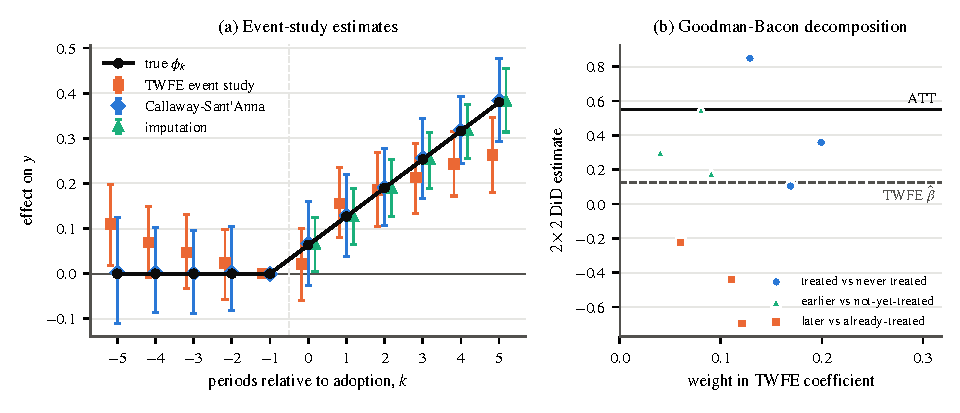
\includegraphics[width=\textwidth]{figures/appA/staggered.pdf}
\caption{Staggered adoption with effects that grow over time and differ across cohorts. (a) Mean estimates
of the event-time effects over 500 replications, with bars from the 5th to the 95th percentile. The black line is
the true effect, averaged over the cohorts observed at each relative time. The TWFE event study includes dummies
for $k=-5,\dots,5$ (omitting $k=-1$) and binned end points. (b) Goodman-Bacon decomposition of the expected
static TWFE coefficient (dashed line). Each marker is one two-by-two comparison. The solid line is the average effect
over all treated unit-periods. The design has 400 units, 20 periods, adoption in periods 5, 10 and 15 plus a never-treated
group. Numbers from \texttt{staggered\_did.py}, seed 20261022.}
\label{fig:A-staggered}
\end{figure}

The lesson for applied work is direct. When treatment timing varies and effects may change with exposure, we
should report heterogeneity-robust estimates alongside, or instead of, TWFE. The Goodman-Bacon decomposition is a
useful diagnostic, because it shows how much weight the forbidden comparisons receive. In merger retrospectives that
pool mergers closing at different dates, and in patent or entry studies with staggered timing, the issue arises
whenever the effect builds up gradually.

\subsection{Related designs}\label{sec:A-did-related}

\casehead{Synthetic control}
Many IO questions concern a single treated unit, such as the local market of one merger or one state's regulation.
With one treated unit, the choice of control group carries the whole design. The \emph{synthetic control} method
\citep{AbadieGardeazabal2003,AbadieDiamondHainmueller2010} builds the control as a weighted average of untreated
units. Let unit 1 be treated after period $T_0$ and units $2,\dots,J+1$ be potential controls. Let $X_1$ be a vector
of pre-treatment characteristics of the treated unit, including pre-period outcomes, and $X_0$ the matrix of the same
characteristics for the controls. The weights solve
\begin{equation*}
\min_{w}\ \big\|X_1-X_0w\big\|_V\quad\text{subject to}\quad w_j\ge0,\ \ \sum_{j=2}^{J+1}w_j=1,
\end{equation*}
for a positive definite weighting matrix $V$ chosen to fit pre-period outcomes. The estimated effect in period
$t>T_0$ is $y_{1t}-\sum_jw_jy_{jt}$. The constraints rule out extrapolation, because the synthetic unit lies in the
convex hull of the controls. The method is credible when the synthetic unit tracks the treated unit closely over a
long pre-period. Inference uses placebo assignments, applying the method to each control unit in turn and comparing
the treated unit's post-period gap with the placebo gaps. \citet{Abadie2021} discusses data requirements and
practice.

\casehead{Triple differences}
When the control group may face different trends, a third difference can remove them. Suppose a merger affects
product category $A$ in region 1, and region 2 and category $B$ are unaffected. The \emph{triple difference} is
\begin{equation*}
\hat\beta^{\mathrm{DDD}}=\big[\Delta\bar y_{A1}-\Delta\bar y_{A2}\big]-\big[\Delta\bar y_{B1}-\Delta\bar y_{B2}\big],
\end{equation*}
where $\Delta\bar y_{cr}$ is the change in the mean outcome of category $c$ in region $r$. The first bracket is a
regional DiD for category $A$. The second removes region-specific trends that also appear in category $B$. The
identifying assumption is that the gap between the regional trends would have been the same in both categories.
This is weaker than parallel trends for either DiD alone.

\casehead{Regression discontinuity}
When treatment is assigned by a known rule based on a running variable $z_i$, with $d_i=\indic\{z_i\ge c\}$, units
just above and just below the cutoff $c$ are comparable. If potential outcomes are continuous in $z$ at $c$, the
jump $\lim_{z\downarrow c}\E[y_i\mid z_i=z]-\lim_{z\uparrow c}\E[y_i\mid z_i=z]$ identifies the average effect at
the cutoff. Estimation uses local linear regression on each side (\cref{sec:A-loclin}). \citet{LeeLemieux2010} survey
the design. \citet{AtheyLevinSeira2011} discuss a deterministic rule for the format of timber sales, such as an open
auction whenever timber volume exceeds a threshold. Under such a rule their comparison would be identified in a
manner analogous to a regression discontinuity design (n.~13, p.~229).

\casehead{Selection on observables and matching}
A different design drops the panel. It assumes \emph{unconfoundedness}, that treatment is as good as random given
observed covariates: $(y_i(0),y_i(1))\perp d_i\mid x_i$. It also assumes \emph{overlap}, $0<\psi(x)<1$, where
$\psi(x)=\Pr(d_i=1\mid x_i=x)$ is the \emph{propensity score}. \citet{RosenbaumRubin1983} show that unconfoundedness given
$x_i$ implies unconfoundedness given $\psi(x_i)$. The proof is short. By iterated expectations,
\begin{equation*}
\Pr\big(d_i=1\mid y_i(0),y_i(1),\psi(x_i)\big)=\E\big[\Pr(d_i=1\mid y_i(0),y_i(1),x_i)\mid y_i(0),y_i(1),\psi(x_i)\big]=\psi(x_i),
\end{equation*}
because the inner probability equals $\psi(x_i)$ by unconfoundedness. Comparisons may therefore condition on the
scalar $\psi$ instead of the whole vector $x$. Estimators include regression adjustment, inverse propensity
weighting and matching. A matching estimator imputes each unit's missing potential outcome by the average outcome of
its $M$ nearest neighbors in the other treatment group. \citet{AbadieImbens2006} derive its large-sample distribution
and a consistent variance estimator. \citet{ImbensRubin2015} give a full treatment.

\citet{AtheyLevinSeira2011} use these tools to compare sealed-bid and open timber auctions held by the US Forest
Service (\cref{ch:auction-empirics}). Their sales took place between 1982 and 1990 in the Northern forests and between
1982 and 1989 in California. For an outcome $Y$ they write $Y=f(\mathit{SEALED},X,N,\epsilon)$
and target the average effect $\Delta Y=\E[f(1,X,N,\epsilon)-f(0,X,N,\epsilon)]$ (eq.~5, p.~229). The identifying
assumption is that the auction format is independent of $\epsilon$ given the covariates. It holds by design for sales
whose format was randomized, and for other sales if the format was chosen on information in their data. They
estimate a logit propensity score of the sealed-bid format on tract characteristics and drop sales with predicted
probabilities below 0.075 or above 0.925 to enforce overlap (p.~227). Their matching estimator is
\begin{equation*}
\widehat{\Delta Y}=\frac{1}{T}\sum_{t\ \text{sealed}}\big(Y_t-\hat Y_t\big)+\frac{1}{T}\sum_{t\ \text{open}}\big(\hat Y_t-Y_t\big)
\end{equation*}
(eq.~7, p.~230). Here $T$ is the number of sales, and $\hat Y_t$ is the average outcome of the $M=4$ sales of the
other format with the closest propensity scores. Standard errors follow \citet{AbadieImbens2006}. \Cref{tab:A-als}
compares the matching estimates with two regression estimates. In the Northern forests the three estimators agree
closely. Sealed bidding raises logger entry by about 10 percent and the sale price by 9 to 12 percent. In
California the price effects are small and insignificant, and the matching estimates are imprecise. Trimming for
overlap kept only a third of the California sales (p.~227). The authors also report similar estimates on the 378 Northern sales whose format
was randomized (p.~226).

\begin{table}[htbp]
\centering
\caption{Effect of sealed bidding on timber sale outcomes: regression and matching}
\label{tab:A-als}
\footnotesize
\begin{tabular}{@{}lcccc@{}}
\toprule
& \multicolumn{2}{c}{Northern forests ($N=1{,}071$)} & \multicolumn{2}{c}{California ($N=707$)}\\
\cmidrule(lr){2-3}\cmidrule(l){4-5}
Estimator & $\ln$(logger entry) & $\ln$(price) & $\ln$(logger entry) & $\ln$(price)\\
\midrule
OLS, no interactions & 0.089 & 0.094 & 0.101 & 0.027\\
 & (0.036) & (0.038) & (0.045) & (0.051)\\
OLS with sealed $\times$ covariate interactions & 0.097 & 0.099 & 0.099 & 0.026\\
 & (0.036) & (0.039) & (0.044) & (0.050)\\
Propensity-score matching, $M=4$ & 0.100 & 0.118 & 0.106 & $-0.038$\\
 & (0.048) & (0.064) & (0.062) & (0.127)\\
\bottomrule
\end{tabular}

\smallskip
\parbox{0.92\linewidth}{\footnotesize Notes: Each entry is the estimated effect of the sealed-bid format, with robust
standard errors in parentheses (Abadie-Imbens standard errors for matching). Regressions control for the Forest
Service appraisal variables, sale characteristics and year, quarter and location dummies. Samples exclude sales with
propensity scores outside $[0.075,0.925]$. Source: \citet{AtheyLevinSeira2011}, Table~III, columns 1 and 5.}
\end{table}

\section{Financial event studies}\label{sec:A-eventstudy}

A financial \emph{event study} measures the effect of a discrete piece of news on the market value of firms. The
method goes back to \citet{FamaEtAl1969}, and \citet{MacKinlay1997} surveys it. Industrial organization uses it to
learn about profits that we cannot observe directly. A merger that raises market power should raise the value of the
merging firms' rivals, and entry into a profitable market should lower the value of incumbents. This section
develops the method in general form. \Cref{sec:09-wc-method} applies it in full to the entry study of
\citet{WhinstonCollins1992}, and \cref{sec:11-retro-event} applies it to mergers.

\subsection{Premise}\label{sec:A-es-premise}

The method rests on \emph{market efficiency}. The equity value of a firm equals the expected present value of the
cash flows to its shareholders, given all public information. When news changes expected future profits, the share
price adjusts as soon as the news becomes public. The return on the announcement day, net of the return the stock
would have earned anyway, then measures the revision in the expected value of the firm to its shareholders. A study
of a few days of returns can thus reveal a change in discounted profits over many years. The price of this economy is
a set of assumptions about information, timing and the model of normal returns, which we make explicit below.

\subsection{Normal returns and abnormal returns}\label{sec:A-es-ar}

Index firms by $f$ and trading days by $\tau$, with the announcement on day $\tau=0$ of \emph{event time}. Let
$R_{f\tau}$ be the return on firm $f$'s stock, including dividends, $R^m_\tau$ the return on a market index and
$R^0_\tau$ the risk-free rate. The \emph{normal return} is the return expected without the event. Three models are
common. The \emph{constant-mean model} sets $R_{f\tau}=\mu_f+u_{f\tau}$. The \emph{market model} sets
\begin{equation}\label{eq:A-es-mm}
R_{f\tau}=a_f+b_f R^m_\tau+u_{f\tau},\qquad \E[u_{f\tau}\mid R^m]=0,\quad \Var(u_{f\tau}\mid R^m)=\sigma_f^2,
\end{equation}
with errors uncorrelated across days. The \emph{excess-return} form of the capital asset pricing model replaces
returns by returns in excess of the risk-free rate,
$R_{f\tau}-R^0_\tau=a_f+b_f(R^m_\tau-R^0_\tau)+u_{f\tau}$, as in \cref{sec:09-wc-method}. The market model removes the
part of the return due to market-wide news, which reduces the variance of the abnormal return and raises power.

The model is estimated on an \emph{estimation window} of $T_e$ trading days that ends some days before the event,
so that the event cannot affect the estimates. The \emph{event window} is $[\tau_1,\tau_2]$, which contains day
0 and has $L=\tau_2-\tau_1+1$ days. Days before the announcement allow for leakage, and days after it allow for slow
absorption. \Cref{fig:A-es-timeline} shows the layout.

\begin{figure}[htbp]
\centering
\begin{tikzpicture}[x=1cm,y=1cm]
\draw[-{Stealth[length=2.4mm]}, thick] (0,0) -- (14.2,0);
\node[font=\footnotesize, anchor=north east] at (14.2,-0.15) {event time $\tau$};
\fill[blue!18] (0.3,-0.14) rectangle (6.3,0.14);
\fill[gray!15] (6.3,-0.14) rectangle (7.9,0.14);
\fill[orange!35] (7.9,-0.14) rectangle (10.3,0.14);
\fill[gray!30] (10.3,-0.14) rectangle (13.4,0.14);
\foreach \x/\lab in {0.3/{\tau_1-g-T_e}, 6.3/{\tau_1-g-1}, 7.9/{\tau_1}, 9.1/{0}, 10.3/{\tau_2}} {
  \draw (\x,0.18) -- (\x,-0.18);
  \node[font=\footnotesize, below] at (\x,-0.2) {$\lab$};
}
\node[font=\footnotesize, anchor=north] at (9.1,-0.62) {(announcement)};
\draw[decorate, decoration={brace, amplitude=5pt}] (0.3,0.3) -- (6.3,0.3)
  node[midway, above=6pt, font=\footnotesize, align=center] {estimation window\\$T_e$ days: estimate $a_f$, $b_f$, $\sigma_f^2$};
\draw[decorate, decoration={brace, amplitude=4pt}] (6.35,0.3) -- (7.85,0.3)
  node[midway, above=5pt, font=\footnotesize] {gap, $g$ days};
\draw[decorate, decoration={brace, amplitude=5pt}] (7.9,0.3) -- (10.3,0.3)
  node[midway, above=6pt, font=\footnotesize, align=center] {event window\\$L$ days};
\draw[decorate, decoration={brace, mirror, amplitude=5pt}] (10.7,-0.85) -- (13.4,-0.85)
  node[midway, below=6pt, font=\footnotesize] {post-event window};
\end{tikzpicture}
\caption{Windows in a financial event study. The normal-return model is estimated on the estimation window, which
ends $g$ days before the event window so that the event cannot affect the estimates. Abnormal returns are computed
on the event window $[\tau_1,\tau_2]$ around the announcement on day 0. A post-event window can be used to check for
slow adjustment.}
\label{fig:A-es-timeline}
\end{figure}

\begin{definition}[Abnormal and cumulative abnormal returns]\label{def:A-es-ar}
Let $(\hat a_f,\hat b_f)$ be the OLS estimates of \eqref{eq:A-es-mm} on the estimation window. The \emph{abnormal
return} on an event-window day is the prediction error
$AR_{f\tau}=R_{f\tau}-\hat a_f-\hat b_fR^m_\tau$. The \emph{cumulative abnormal return} is
$CAR_f(\tau_1,\tau_2)=\sum_{\tau=\tau_1}^{\tau_2}AR_{f\tau}$.
\end{definition}

The variance of abnormal returns has a compact matrix form. Stack the estimation-window data as $y_e$ ($T_e\times1$)
and $X_e=[\iota,\,R^m_e]$ ($T_e\times2$), and the event-window data as $y^*$ ($L\times1$) and $X^*$ ($L\times2$). Let
$AR^*$ be the $L\times1$ vector of abnormal returns.

\begin{proposition}[Variance of abnormal returns]\label{prop:A-es-arvar}
Suppose that \eqref{eq:A-es-mm} holds on both windows under the null hypothesis of no event effect. Let the errors
be independent of the market returns and uncorrelated across days, with variance $\sigma_f^2$. Then, conditional on
the market returns,
\begin{equation*}
\E\big[AR^*\big]=0,\qquad \Var\big(AR^*\big)=\sigma_f^2\Big[I_L+X^*(X_e^\top X_e)^{-1}X^{*\top}\Big].
\end{equation*}
For a single day,
\begin{equation*}
\Var\big(AR_{f\tau}\big)=\sigma_f^2\left[1+\frac{1}{T_e}+\frac{(R^m_\tau-\hat\mu_m)^2}{\sum_{s}(R^m_s-\hat\mu_m)^2}\right],
\end{equation*}
where $\hat\mu_m$ is the mean market return over the estimation window and the sum runs over it. For the
cumulative abnormal return, $\Var(CAR_f)=\iota^\top\Var(AR^*)\,\iota$.
\end{proposition}

\begin{proof}
Write $\theta_f=(a_f,b_f)^\top$ and $\hat\theta_f=(X_e^\top X_e)^{-1}X_e^\top y_e$. Under the null,
$y^*=X^*\theta_f+u^*$, so
\begin{equation*}
AR^*=y^*-X^*\hat\theta_f=u^*-X^*(\hat\theta_f-\theta_f)=u^*-X^*(X_e^\top X_e)^{-1}X_e^\top u_e .
\end{equation*}
Both terms have mean zero. The event-window errors $u^*$ are uncorrelated with the estimation-window errors $u_e$,
so the variance is the sum of $\Var(u^*)=\sigma_f^2I_L$ and
\begin{equation*}
X^*(X_e^\top X_e)^{-1}X_e^\top\Var(u_e)X_e(X_e^\top X_e)^{-1}X^{*\top}=\sigma_f^2X^*(X_e^\top X_e)^{-1}X^{*\top}.
\end{equation*}
For a single day with regressor row $x_\tau=(1,R^m_\tau)$, write $Q=\sum_s(R^m_s-\hat\mu_m)^2$. The inverse is
\begin{equation*}
(X_e^\top X_e)^{-1}=\frac{1}{T_eQ}\begin{pmatrix}\sum_s(R^m_s)^2 & -\sum_sR^m_s\\ -\sum_sR^m_s & T_e\end{pmatrix}.
\end{equation*}
Then $x_\tau(X_e^\top X_e)^{-1}x_\tau^\top=\frac{\sum_s(R^m_s)^2-2R^m_\tau\sum_sR^m_s+T_e(R^m_\tau)^2}{T_eQ}$.
Substituting $\sum_s(R^m_s)^2=Q+T_e\hat\mu_m^2$ and $\sum_sR^m_s=T_e\hat\mu_m$, the numerator becomes
$Q+T_e(R^m_\tau-\hat\mu_m)^2$. Dividing by $T_eQ$ gives $\frac{1}{T_e}+\frac{(R^m_\tau-\hat\mu_m)^2}{Q}$. The variance
of the cumulative abnormal return is the variance of $\iota^\top AR^*$.
\end{proof}

The term $X^*(X_e^\top X_e)^{-1}X^{*\top}$ is estimation error in the normal-return model. It vanishes as $T_e$
grows, and with a typical estimation window of a year of trading days it is small. Its off-diagonal elements are not
zero, so abnormal returns on different event-window days are correlated through the common estimation error.

\casehead{Test statistics}
Replacing $\sigma_f^2$ by the residual variance $\hat\sigma_f^2=\frac{1}{T_e-2}\sum_s\hat u_{fs}^2$ gives the
\emph{standardized cumulative abnormal return}
\begin{equation*}
SCAR_f=\frac{CAR_f(\tau_1,\tau_2)}{\widehat{\mathrm{sd}}\big(CAR_f\big)} .
\end{equation*}
Under normal errors and the null it has a $t$ distribution with $T_e-2$ degrees of freedom, and it is approximately
standard normal for long estimation windows. With $N$ events on different calendar dates the abnormal returns are
independent across events. Two aggregate statistics are standard. The first divides the average CAR,
$\overline{CAR}=\frac{1}{N}\sum_fCAR_f$, by $\frac{1}{N}(\sum_f\widehat{\Var}(CAR_f))^{\frac{1}{2}}$. The second
averages the standardized values. A $t$ variable with $T_e-2$ degrees of freedom has variance $\frac{T_e-2}{T_e-4}$, so
\begin{equation*}
\Big(\frac{N(T_e-4)}{T_e-2}\Big)^{\frac{1}{2}}\,\frac{1}{N}\sum_{f=1}^{N}SCAR_f\ \xrightarrow{d}\ N(0,1)
\end{equation*}
as $N$ grows. The second statistic weights events with volatile stocks less.

\casehead{Power and the length of the window}
A short window raises power. Suppose an event moves the value by a fraction $A$ spread over an $L$-day window, and
ignore estimation error. The expected standardized CAR of one event is about $\frac{A}{\sigma_f\sqrt L}$. With daily
volatility $\sigma_f=0.02$ and $A=0.01$, it is 0.5 for a one-day window. With $N=50$ independent events the aggregate
statistic is about $0.5\sqrt{50}\approx3.5$. With an eleven-day window the same effect gives about
$\frac{3.5}{\sqrt{11}}\approx1.07$, which is insignificant. \citet{BrownWarner1985} study the properties of these
tests with daily data.

\casehead{Events on the same date}
When several firms are hit by the same news, their abnormal returns are correlated. Industry news that the market
index does not absorb moves them together. Suppose $N$ firms share an event date, each CAR has variance $v$, and each
pair has correlation $\rho$. Then
\begin{equation*}
\Var\big(\overline{CAR}\big)=\frac{1}{N^2}\big[Nv+N(N-1)\rho v\big]=\frac{v}{N}\big[1+(N-1)\rho\big],
\end{equation*}
the same inflation factor as in clustered regressions (\cref{prop:A-moulton}). One remedy is the \emph{portfolio
approach}. We form an equally weighted portfolio of the affected firms, estimate the market model for the portfolio
return, and compute its abnormal return. The portfolio residual variance estimates
$\frac{1}{N^2}\iota^\top\Sigma\iota$ directly, so the covariance is accounted for. The other remedy, a system of
regressions, follows.

\subsection{Regression form}\label{sec:A-es-regression}

The two-step procedure has an equivalent one-step form. We estimate the market model on the estimation and event
windows together and add one indicator for each event-window day:
\begin{equation}\label{eq:A-es-dummy}
R_{f\tau}=a_f+b_fR^m_\tau+\sum_{s=\tau_1}^{\tau_2}\gamma_{fs}\,\indic\{\tau=s\}+u_{f\tau}.
\end{equation}

\begin{proposition}[Dummy-variable form]\label{prop:A-es-dummy}
OLS on \eqref{eq:A-es-dummy} gives the estimation-window estimates $(\hat a_f,\hat b_f)$, and
$\hat\gamma_{fs}=AR_{fs}$ for every event-window day $s$. Under the assumptions of \cref{prop:A-es-arvar}, the
conventional OLS variance of $(\hat\gamma_{f\tau_1},\dots,\hat\gamma_{f\tau_2})$ equals $\Var(AR^*)$.
\end{proposition}

\begin{proof}
Order the observations with the estimation window first. The regressor matrix and the dummy matrix are
\begin{equation*}
X=\begin{pmatrix}X_e\\X^*\end{pmatrix},\qquad Q_d=\begin{pmatrix}0\\I_L\end{pmatrix}.
\end{equation*}
By the Frisch-Waugh-Lovell theorem
(\cref{thm:A-fwl}), the coefficients on $X$ equal those from regressing $M_{Q}y$ on $M_{Q}X$, where
$M_Q=I-Q_d(Q_d^\top Q_d)^{-1}Q_d^\top$. This annihilator sets the event-window rows to zero and leaves the
estimation-window rows unchanged. The regression therefore uses only estimation-window data, and its coefficients are
$(\hat a_f,\hat b_f)$. The dummy coefficients solve the remaining normal equations,
$Q_d^\top(y-X\hat\theta_f-Q_d\hat\gamma_f)=0$, which give $\hat\gamma_f=y^*-X^*\hat\theta_f=AR^*$. Each dummy fits its
observation exactly.

For the variance, the FWL theorem gives the conventional variance of $\hat\gamma_f$ as
$\sigma_f^2(Q_d^\top M_XQ_d)^{-1}$, with $M_X=I-X(X^\top X)^{-1}X^\top$. Now $Q_d^\top M_XQ_d=I_L-X^*(X^\top X)^{-1}X^{*\top}$
and $X^\top X=X_e^\top X_e+X^{*\top}X^*$. The Woodbury identity gives
\begin{equation*}
\Big[I_L-X^*\big(X_e^\top X_e+X^{*\top}X^*\big)^{-1}X^{*\top}\Big]^{-1}=I_L+X^*(X_e^\top X_e)^{-1}X^{*\top}.
\end{equation*}
So the conventional variance equals $\sigma_f^2[I_L+X^*(X_e^\top X_e)^{-1}X^{*\top}]$, which is $\Var(AR^*)$.
\end{proof}

The regression form has three advantages. The sum of the dummy coefficients is the CAR, and its standard error comes
from the regression. A single dummy for all window days estimates the average daily abnormal return directly, and
$L$ times it estimates the cumulative effect. And the event effect can depend on firm and event characteristics,
which lets many firms and events be estimated jointly. \Cref{prop:09-wc-dummy} gives the scalar version used by
Whinston and Collins.

\casehead{Systems of firms}
With $M$ firms observed on the same days, we stack the firm equations for day $\tau$ as
$y_\tau=X_\tau\theta+u_\tau$. The vector $\theta$ may contain parameters common to all firms, such as the effect of an
event per unit of exposure. A
system of \emph{seemingly unrelated regressions} (SUR) allows errors to be correlated across firms on the same day
and uncorrelated across days, $\E[u_\tau u_\tau^\top]=\Sigma$ \citep{Zellner1962}. Feasible GLS estimates $\Sigma$
from first-stage residuals (\cref{sec:A-systems}). \citet[pp.~170--173]{Binder1985} applies this system, which he calls
the multivariate regression model, to regulatory events that affect many firms at once.
GLS reduces to equation-by-equation OLS when every equation has the
same regressors and no parameter is shared (\cref{prop:A-sur-ols}). Binder's system meets both conditions, since each
firm has its own abnormal returns and all equations share one regressor matrix. In his system the GLS point estimates
therefore equal OLS, and SUR matters for his tests across firms, whose statistics use $\hat\Sigma$ (p.~173). Neither condition holds when the event effect is
a common parameter scaled by firm-specific exposure, and SUR then gains efficiency and gives standard errors that
account for same-day correlation. \citet{WhinstonCollins1992} estimate such a system for a panel of 20 airlines,
People Express included, ``allowing the $\{\epsilon_{it}\}$ to be contemporaneously correlated across firms''
(p.~449).

\casehead{Dollar abnormal values}
An abnormal return measures the event's effect relative to the firm's value. The \emph{dollar abnormal value} on day
$\tau$ is $V_{f,\tau-1}AR_{f\tau}$, where $V_{f,\tau-1}$ is the equity value at the previous close. Summing over the
window gives the change in shareholder wealth. The choice between returns and dollars is a modelling choice about the
event. If the event changes the firm's value by a fixed dollar amount $\Delta_f$, its return effect is
$\frac{\Delta_f}{V_{f,\tau-1}}$. A model with a common abnormal return across firms would then force larger firms
to have proportionally larger dollar effects. Whinston and Collins argue that the loss from being an incumbent in one
entered market should not scale with the carrier's size (p.~449). They therefore model dollar effects, with the
return equation
\begin{equation*}
R_{f\tau}-R^0_\tau=\frac{a_f}{V_{f,\tau-1}}+b_f\big(R^m_\tau-R^0_\tau\big)+\frac{\Delta_f(Z_\tau)}{V_{f,\tau-1}}+u_{f\tau},
\end{equation*}
where $\Delta_f(Z_\tau)$ is the dollar effect of the events on day $\tau$ (\cref{eq:09-wc-dollar}). Estimating in
return units keeps the error homoskedastic. The equivalent dollar regression would have errors with variance
$V_{f,\tau-1}^2\sigma_f^2$. Their simplest specification makes the dollar loss proportional to the incumbent's
annualized seatmiles on the entered route. The estimated loss per seatmile is $-0.0109$ (s.e.\ 0.0035) for a one-day
window, $-0.0147$ (0.0049) for two days and $-0.0191$ (0.0061) for three days (Table~1, p.~453). These are total
changes over each window. They imply losses of \$3.7 million to \$6.5 million per incumbent (p.~452). \Cref{tab:09-wc-t1}
reports the full results.

\subsection{Identification and pitfalls}\label{sec:A-es-pitfalls}

An abnormal return equals the change in expected shareholder value caused by the event only under several
conditions. Each can fail in IO applications.

\casehead{Dating and leakage}
The event must be dated by the first public report. News often leaks before formal announcements, through
rumors, regulatory filings or trade press. Longer windows capture leakage but add the noise of unrelated news on each
extra day, and by the power calculation above they dilute the test. Whinston and Collins date each event by the
earliest report in the trade or financial press, and use one-, two- and three-day windows ending on that day
(p.~450).

\casehead{Anticipation}
Markets price events before they happen when they expect them. The next result makes the consequence precise.

\begin{proposition}[Partial anticipation]\label{prop:A-es-anticipation}
Suppose that before the announcement the market assigns probability $\pi$ to an event that would change the firm's
value by $\Delta V$, and that the announcement resolves the uncertainty. If the event is announced, the measured
value change is $(1-\pi)\Delta V$. If the announcement reveals that the event will not happen, the measured change is
$-\pi\Delta V$.
\end{proposition}

\begin{proof}
Let $V^0$ be the value without the event. Before the announcement the value is the expectation
$V^0+\pi\Delta V$. If the event is announced, the value becomes $V^0+\Delta V$, and the change is
$(V^0+\Delta V)-(V^0+\pi\Delta V)=(1-\pi)\Delta V$. If the event is ruled out, the value becomes $V^0$, and the change
is $-\pi\Delta V$.
\end{proof}

Announcement returns therefore understate the value of events that were partly expected, and the bias is larger the
more predictable the event. Dividing by $1-\pi$ corrects the estimate if $\pi$ is known.
\citet[pp.~240--241]{MalatestaThompson1985} show that $\pi$ need not be known when events of constant expected value recur with a
constant probability per period. Repeated acquisition attempts by one firm are an example. They regress the firm's dollar excess
return on a market term and a dummy for periods with an event. The intercept then estimates $-\pi\Delta V$, and the
dummy coefficient estimates $\Delta V$ itself.
A merger announcement raises the probability of the
merger, and an antitrust complaint lowers it. Under \cref{prop:A-es-anticipation} the two events move the rivals'
values in opposite directions with magnitudes that depend on the prior probabilities. This is the logic behind the
rival tests in \cref{tab:11-eventpred}.

\casehead{Information revealed by the event}
An event can reveal information beyond its direct effect. A merger announcement may reveal that scale economies are
available to the whole industry, or that rivals are attractive targets. Rivals' values then rise for reasons other
than market power. Entry by one firm may reveal its plans for further expansion. Whinston and Collins find
industry-wide losses that they cannot fully attribute, and list such informational effects among the possible
sources (p.~448).

\casehead{Confounding events and calendar clustering}
Other news inside the window that is correlated with exposure to the event biases the estimate. Events that cluster
on the same dates create the cross-sectional dependence discussed above. Event-induced changes in volatility make the
estimation-window variance too small. A test that standardizes each abnormal return and then uses the cross-sectional
variance of the standardized values guards against this \citep{BoehmerMusumeciPoulsen1991}.

\casehead{Thin trading}
Stocks that trade infrequently have stale prices, which biases estimated betas and spreads the response over
several days. Estimators that use leads and lags of the market return correct the betas \citep{ScholesWilliams1977}.

\casehead{Who captures the change}
Equity values measure only the shareholders' part of a change in firm value. Part of the rents from market power can
accrue to debtholders, to workers through rent sharing, or to managers. Whinston and Collins note that misdating,
partial anticipation, and value changes felt by debtholders or workers all bias their estimates toward zero
(p.~453). Effects on consumers do not appear in stock prices at all, so an event study measures only producer gains
and losses.

\subsection{Uses in industrial organization}\label{sec:A-es-io}

\casehead{Mergers}
The value created for the merging firms combines market power and efficiencies, so it cannot tell them apart. The
returns of rivals can. A merger that raises prices raises rivals' profits, while a merger that creates a more
efficient competitor lowers them. \citet{Eckbo1983} and \citet{Stillman1983} compare rivals' abnormal returns at the
merger announcement and at the antitrust complaint. Under the market-power hypothesis the two returns have opposite
signs, positive and then negative. \Cref{tab:11-eventpred} lists the predictions, including the information
hypothesis that weakens the test. The design also needs rivals that are publicly traded and for which the affected
market is a large part of value. \Cref{sec:11-retro-event} discusses applications and their limits.
\citet[p.~231, n.~137]{AskerNocke2021} report that most authors doubt that an event study can reveal the competitive
effects of one specific merger. In their reading the method works best for patterns across large samples of mergers.

\casehead{Entry and contestability}
Incumbents' value losses at an entry announcement reveal profits or sunk costs on the entered route, which perfect
contestability rules out. \citet{WhinstonCollins1992} use differences in exposure across carriers to separate three
sources of loss (\cref{sec:09-wc}). These are incumbency on the entered airport pair, presence at other airports of
the same city pair, and general effects felt by all carriers. The panel DiD of \cref{sec:A-did-control} then checks the mechanism with
prices, quantities and capacity.

\casehead{Regulation}
Regulatory events change the profits of whole industries at once. \citet[p.~448, n.~5]{WhinstonCollins1992} cite
\citet{Schwert1981} and \citet{Rose1985} as earlier uses of the event study in industrial organization. Their titles
are ``Using Financial Data to Measure the Effects of Regulation'' (Schwert) and ``The Incidence of Regulatory Rents in
the Motor Carrier Industry'' (Rose).
\citet[pp.~168--169]{Binder1985} applies the multivariate regression model to 20 major regulatory changes between 1887 and 1978.
News about each change came out in 5.6 announcements on average, spread over 18.5 months (p.~170). His tests reject
the null of no abnormal returns only slightly more often than chance would predict (p.~174). He concludes that the
formal announcements were generally anticipated (p.~181).
Because regulatory news is often anticipated and spread over many dates,
\cref{prop:A-es-anticipation} and the dating problem are especially relevant here.

The financial event study and the panel DiD answer related questions with different data. The first measures
expected changes in producer value at the moment of the news. The second measures realized changes in prices and
quantities over months or years. Studies that use both, as Whinston and Collins do, can check one against the other.
